%                                                                 aa.dem
% AA vers. 8.2, LaTeX class for Astronomy & Astrophysics
% demonstration file
%                                                       (c) EDP Sciences
%-----------------------------------------------------------------------
%
%\documentclass[referee]{aa} % for a referee version
%\documentclass[onecolumn]{aa} % for a paper on 1 column  
%\documentclass[longauth]{aa} % for the long lists of affiliations 
%\documentclass[rnote]{aa} % for the research notes
%\documentclass[letter]{aa} % for the letters 
%\documentclass[bibyear]{aa} % if the references are not structured 
% according to the author-year natbib style

%
\documentclass[referee]{aa}  

%
\usepackage{graphicx}
\usepackage{caption}
\usepackage{subcaption}
%%%%%%%%%%%%%%%%%%%%%%%%%%%%%%%%%%%%%%%%
\usepackage{txfonts}
%%%%%%%%%%%%%%%%%%%%%%%%%%%%%%%%%%%%%%%%
%\usepackage[options]{hyperref}
% To add links in your PDF file, use the package "hyperref"
% with options according to your LaTeX or PDFLaTeX drivers.
%
% Enable mutiple title row on tables.
\usepackage{multirow}
%%%%%%%%%%%
% 
% Dealing with ``too many unprocessed floats'' use it with \clearpage 
\usepackage[section] {placeins}

% For marginal notes
\usepackage{marginnote}

\begin{document} 


   \title{Physical parameter estimates of M-type stars: a machine learning perspective.}

   \author{
          J. Ordieres-Mere \inst{2} 
          \and
          A. Bello-Garcia\inst{3} 
          \and
          A. Gonzalez-Marcos\inst{4} 
          \and
          M.B. Prendes-Gero\inst{3} 
          \and
          L. M. Sarro \inst{1}  
          }

   \institute{ 
      \inst{1} Universidad Nacional de Educaci\'{o}n a Distancia, \\
               Department of Artificial Intelligence.
               \email{lsb@uned.es}
        \and 
      \inst{2}  Universidad Polit\'{e}cnica de Madrid (UPM), PMQ Research Group, \\
              Jos\'{e} Guti\'{e}rrez Abascal 2, 28006 Madrid, Spain. 
              \email{j.ordieres@upm.es}
        \and 
      \inst{3}   Universidad de Oviedo, Construction and Manufacturing Engineering Department, \\
              Campus de Viesques s/n, Gij\'{o}n, Asturias, Spain. 
              \email{\{abello,mbprendes\}@uniovi.es} 
        \and 
      \inst{4}  Universidad de la Rioja, P2ML Research Group, \\
              Luis de Ulloa 20, 26004 Logro\~{n}o, La Rioja, Spain. 
              \email{ana.gonzalez@unirioja.es}
      }

   \date{Received \today; accepted }

% \abstract{}{}{}{}{} 
% 5 {} token are mandatory
 
  \abstract
  % context heading (optional)
  % {} leave it empty if necessary  
%    {To investigate the physical nature of the `nuc\-leated instability' of
%    proto giant planets, the stability of layers
%    in static, radiative gas spheres is analysed on the basis of Baker's
%    standard one-zone model.}
%   % aims heading (mandatory)
%    {It is shown that stability
%    depends only upon the equations of state, the opacities and the local
%    thermodynamic state in the layer. Stability and instability can
%    therefore be expressed in the form of stability equations of state
%    which are universal for a given composition.}
%   % methods heading (mandatory)
%    {The stability equations of state are
%    calculated for solar composition and are displayed in the domain
%    $-14 \leq \lg \rho / \mathrm{[g\, cm^{-3}]} \leq 0 $,
%    $ 8.8 \leq \lg e / \mathrm{[erg\, g^{-1}]} \leq 17.7$. These displays
%    may be
%    used to determine the one-zone stability of layers in stellar
%    or planetary structure models by directly reading off the value of
%    the stability equations for the thermodynamic state of these layers,
%    specified
%    by state quantities as density $\rho$, temperature $T$ or
%    specific internal energy $e$.
%    Regions of instability in the $(\rho,e)$-plane are described
%    and related to the underlying microphysical processes.}
%   % results heading (mandatory)
%    {Vibrational instability is found to be a common phenomenon
%    at temperatures lower than the second He ionisation
%    zone. The $\kappa$-mechanism is widespread under `cool'
%    conditions.}
%   % conclusions heading (optional), leave it empty if necessary 
   {}

   \keywords{class M stars --
                dynamic feature selection --
                physical parameter identification --
                Temperature, gravity and metalicity Modelling --
                Learning from BT-Settl spectra library
               }

   \maketitle
%

\section{Introduction}
\label{sec:intro}

% The importance of M stars
% The problem of estimation of stellar parameters in the M regime: bands, no continuum...
% who and what. Teff calibrations
% \cite{rajpurohit}
% \cite{amelia}

% Atlases 
%\cite{2013arXiv1306.3709B} % for lambda > 1.1 um :(
%\cite{2009ApJS..185..289R} %IRTF library of cool star

%\cite{2012ApJ...748...93R} % Metall. and Teff indicators in the K band! :(

% Summary of spectral diagnostics in the IR for M stars


\section{Regression models for physical parameter estimation.}

\subsection{Methodology for spectral band selection.}

% Comment. I move the description of the IRTF data to the point where these are actually used.

{ The objective addressed in this Section is to develop a procedure to
  identify spectral bands that yield good temperature, gravity and
  metallicity diagnostics. Given the lack of a calibration set of
  observed spectra with homogeneous coverage of the space of physical
  parameters, we turn to synthetic libraries of spectra. The atomic or
  molecular line/band parameters could in principle indicate the
  spectral features that are more sensitive to changes in the physical
  parameters. The suitability of spectral features as diagnostics
  ofthe stellar atmospheric properties depends not only on the
  individual behaviour of each line/band, but also on the relative
  properties of neighbouring features in the same spectral region,
  that may overlap depending on the spectral resolution. Furthermore,
  good spectral diagnostics at a given signal-to-noise ratio (SNR) may
  show a severy degraded predictive power in the low SNR regime. In
  the following we adopt the BT-Settl library of synthetic spectra
  (\cite{2013MSAIS..24..128A}) as the framework where spectral
  diagnostics will be searched for. These synthetic spectra were
  pre-processed in several steps as described below.}

{ First, and in order to define good temperature diagnostics, spectra
between 2000 and 4200K in steps of 100 K were selected, with $\log(g)$
in the range between 4 and 6 dex (when g is expressed in cm/s$^{-2]$),
in steps of 0.5 dex. The metallicity of the representative spectra was
restricted to the set 0, 0.5 and -1 dex.  This yields a total set
size of 535 available spectra.

The spectral resolution was degraded to the IRTF resolution factor (R
~ 2000) by convolving with a Gaussian. Then, the spectra were trimmed
to produce valid segments between 8145.92 and 24106.85{\AA}, which is
the spectral range common to all M stars in the IRTF library. Finally,
all spectra were divided by the total integrated flux in this range in
order to factor out the stellar distance.}


{ In order to increase the density of examples in parameter space, we
  introduced interpolated spectra in the BT-Settl grid. Interpolation
  was obtained as a linear combination of spectra in the grid,
  weighted by the inverse square of the euclidean distance. {\bf Aqui,
  la distancia euclidea deberia calcularse en parametros normalizados,
  porque si no la temperatura domina la distancia. Fue asi?} We
  compared a set of interpolated spectra with those produced using the
  PHOENIX code (\cite{fuhrmeister2005phoenix}) to be sure that
  interpolation was a valid solution to infer new synthetic
  spectra. {\bf Yo aqui daría el RMSE de reconstruccion, mejor que la
  figura comp-gen-inter}

%(see Fig.~\ref{fig:comp_gen_inter}).  }

%\begin {figure}
% \begin{center}
% 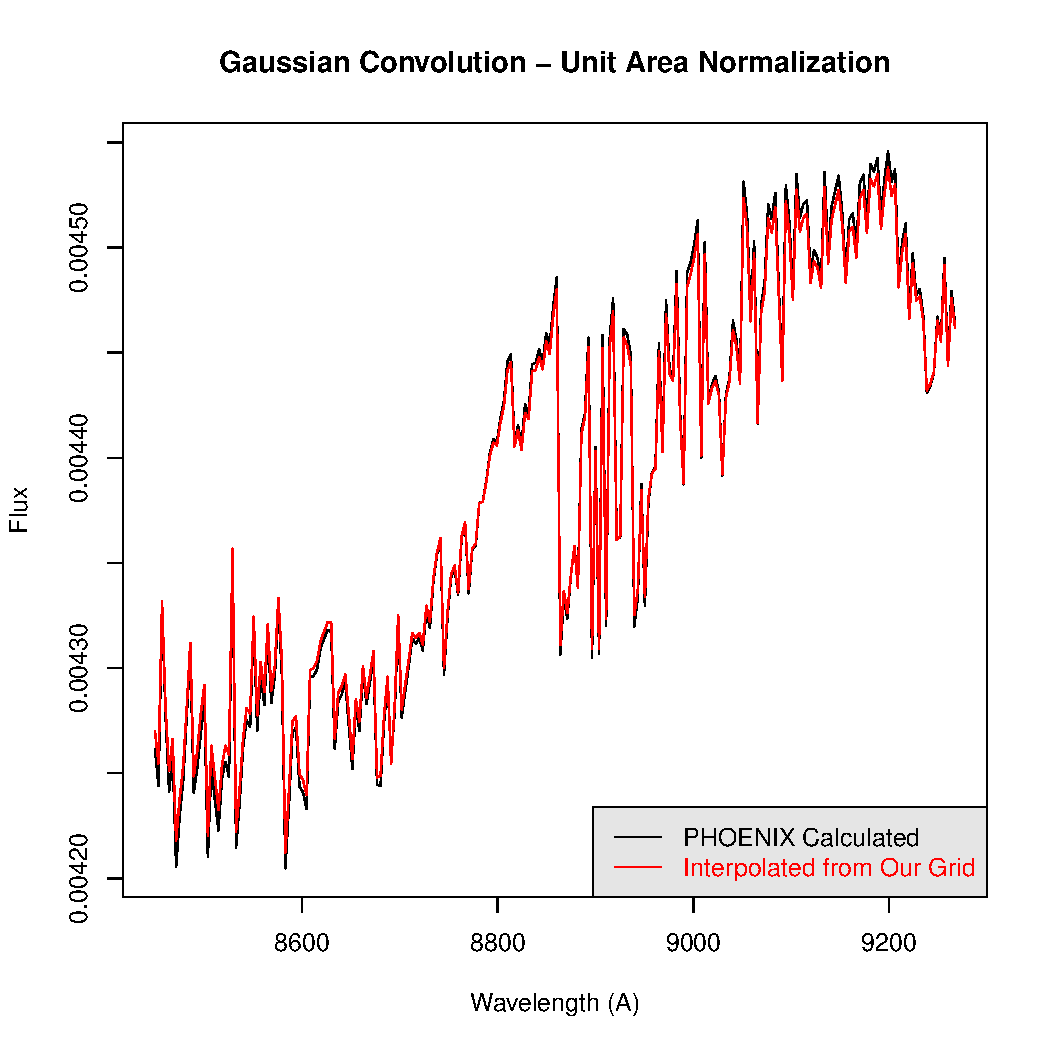
\includegraphics[width=6cm]{figs/intgrid4_gauss.pdf}
% \caption{Comparison between generated and interpollated spectrum}
% \label{fig:comp_gen_inter}
% \end{center}
%\end {figure}

{ A first interpolation stage allowed us to define a finer mesh step of
0.25 dex for both, $\log(g)$ and metallicity and 50K in temperature,
yielding a total 1329 spectra.  Then, a second interpolation stage
refined the grid down to 25 K in temperature and 0.125 dex in 
$\log(g)$, keeping the metallicity step at 0.25 dex and producing a
dataset with 25912 spectra.}

{In spite of these, and in order to keep their knowledge closer to the
original BT-Settl source, most of the analyses have been performed
with the original 535 spectra dataset.  }{\bf Habría que delimitar
exactamente donde se han utilizado 535 y dónde 25912. Si la mayoria
del analisis se ha realizado sobre 535, no se si tiene sentido incluir
la parte de interpolacion.}


{ In order to avoid selecting spectral features that are good
  predictors only in the unrealistic SNR=$\infty$ regime, the search
  for optimal diagnostics of the atmopheric paramters of M stars was
  carried out for three SNR values (10, 50 and $\infty$) by degrading
  the synthetic spectra with Gaussian noise of zero mean.  {\bf Quizás
  deberíamos citar el trabajo de Ana como in preparation} }

\subsection{Feature definition and selection}
\label{subsec:FD}
{ As mentioned in Sect. \ref{sec:intro}, it is well known the
difficulty in defining good spectral diagnostics for M stars in the
infrared.}

{The work in \cite{2013A&A...549A.129C} defined wavelength regions in
the I and K bands optimal for the disagnostic of physical parameters
based on the sensitivity exhibited by the flux emitted in these
segments to changes of the physical parameters. The sensitivity was
measured in terms of the derivative of the flux with respect to the
physical parameter. The approach adopted in this work was to define
the spectral features as those producing the best estimates of
$T_{eff}$, $\log(g)$ and the metallicity. The accuracy of the
estimates produced from a subset of features is established from
regression models described further below.

We consider the effective temperature as the dominant parameter
influencing changes in the stellar spectra (a strong feature) and
thus, it was estimated first, and then used as  in the regression models for the
gravity and metalicity.

The central contribution of this paper is the way to identify the most suitable
regions of spectrum (features) to be considered as signal providers 
but mainly the regions to be considered 
as candidates for being continuum for those signal regions.
It will be performed by means of artificial intelligence techniques.

These features consist of
a central bandpass covering the interesting lines and another bandpass
referring to the local continuum. Then, the feature can be written like 
Eq.~\eqref{eq:feature}.

\begin{equation}\label{eq:feature}
  F(i) =  \frac{ \int_{\lambda_{1s}(i)}^{\lambda_{2s}(i)} \left(f(\lambda)\right) d{\lambda}}
               { \int_{\lambda_{1c}(i)}^{\lambda_{2c}(i)} \left(f(\lambda)\right) d{\lambda}} 
               \quad \quad \forall i \in [1 \ldots N]
\end{equation}


where:
\begin{itemize}
 \item {N means the number of features to be considered, as decided by the researcher.}
 \item {$f(x)$ denotes the normalized flux spectra from the star.}
 \item {$(\lambda_{1s},\lambda_{2s})$ {\AA} accounts for the region of spectrum where the signal is considered. \quad \label{eq:cons1}}
 \item {$(\lambda_{1c},\lambda_{2c})$ {\AA} accounts for the region of spectrum where the continuum is considered.}
\end{itemize}

{
Now, the research question is how to identify 
$\{\lambda_{1s}(i),\lambda_{2s}(i), \lambda_{1c}(i),\lambda_{2c}(i)\}  \quad \forall i \in [1 \ldots N] $
in such a way they become useful to estimate the physical parameters.

Some constaints were estabished as designing of the selection process:

\begin{itemize}
 \item { $ \vert \lambda_{2k(i)} - \lambda_{1k(i)} \vert = 30 $ pixels of spectrum $ \quad \forall i \in [1 \ldots N]$ and $ k \in \{s,c\} $ .}
 \item { $ min ( \lambda_{1k(i)}, \lambda_{1k(j)} ) = 5 $ pixels of spectrum $ \quad \forall i,j \in [1 \ldots N] $ ; $ i \neq j $ and $ k \in \{s,c\} $ .}
 \item { $ \overline{\lambda_{2}(i)\lambda_{1}(i)}  \bigcap 
                      \overline{\lambda_{2c}(i)\lambda_{1c}(i)} = \emptyset \quad \forall i \in [1 \ldots N]$.}
\end{itemize}

which become a guarantee avoiding any overlap 
and a minimum size for both signal and continuum bandpasses.
}

{
Search for those features will depend on which specific physical parameter is 
under consideration but, the proposed methodology will look for those values 
trying to solve an optimization problem, which shall be the forecast capabilities
of one specific set of features, to be retained when it becomes bigger than 
a threshold.

To accomplish such optimization problem involving the selection of variable 
subsets, the use of the Genetic Algorithms technique was accepted. 
}

{ It was proposed to use the software tools R(\cite{R2013}).  There
  are different statistics to identify features that are
  differentially expressed between two or more groups of samples and
  then uses the most differentially expressed to construct a
  statistical model.  }

{ These methods have demonstrated to perform well, however, in some
  cases they can be ineffective regardless of the classification
  method used. An obvious conceptual limitation of univariate
  approaches is also the lack of consideration that features works in
  the contexts of interconnected pathways and therefore it is their
  behavior as a group that may be predictive of the phenotypic
  variables. Multivariate selection methods may seem to be more
  suitable for the analysis of data since variables are tested in
  combination to identify interactions between features. However, the
  extremely large number of models that can be constructed from
  different combination of thousands of features cannot be extensively
  evaluated using standard computational resources.  }

{ For the sake of simplicity let us define Genetic Algorithms (GAs)
  are variable search procedures that are based on the principle of
  evolution by natural selection. The procedure works by evolving sets
  of variables (chromosomes) that fit certain criteria from an initial
  random population via cycles of differential replication,
  recombination and mutation of the fittest chromosomes. The concept
  of using in-silico evolution for the solution of optimization
  problems has been introduced by John Holland in 1975
  (\cite{holland1975adaptation}). Although their application has been
  reasonably widespread (see Goldberg\textquoteright s book
  (\cite{goldberg1989genetic}), they became very popular only when
  sufficiently powerful computers became available.  }

{
The implementation of the GA follows the next steps:
\begin{itemize}
 \item [\textbf{Stage 1}:]{To produce the population of potential features (chromosomes).}
 \item [\textbf{Stage 2}:]{Each chromosome in the population is evaluated for its ability to
predict the group membership of each sample in the dataset (fitness function).}
 \item [\textbf{Stage 3}:]{Chromosome preselection, when a chromosome has 
 a score higher then a predefined value.}
 \item [\textbf{Stage 4}:]{The population of chromosomes is replicated. 
 Chromosomes with a higher fitness score will 
 generate a more numerous offspring.}
 \item [\textbf{Stage 5}:]{The genetic information contained in the replicated parent
chromosomes is combined through genetic crossover. Two randomly selected
parent chromosomes are used to create two new chromosomes.}
 \item [\textbf{Stage 6}:]{Mutations are then introduced in the chromosome randomly. 
 These mutations produce that new genes are used in chromosomes.
 Steps 5 and 6 are applied over the chromosomes establised at Step 4.}
  \item [\textbf{Stage 7}:]{This process is repeated from Stage 2 until 
  enough accuracy is obtained or the maximum of iterations is attained.}
\end{itemize}

The features were constructed as indicated above and named according
to the ordinal of the wavelength step both for signal and
continuum. The name includes also the number of ofset induced because
of the constraint \ref{eq:cons1}.  Polulation size was choosed as one
thousand individuals and accepted iterations were four thousand.
Three randomly started different repetions where produced bringing the
opportunity for enough variety and probabilities were established as
0.85 to corossover and 0.35 to mutation. The elitism was fixed to be
0.15.  Fitness for features were established as related to the Akaike
Criterion (-AIC) for linearity between the potential feature against
the physical parameter.  The most frequent and efficient features were
suggeswted as candidates to describe the behavior of specific physical
parameters.

From the implementation point of view a binarized codification was
selected in accordance to the naming convention and in order to speed
up the computation, a parallel implementation from a farm of fifteen
connected computers were used for each of the physical parameters.  }


{ The GA procedure provides us with a large collection of chromosomes.
  Although these are all potential solutions of the problem, it is not
  clear which one should be chosen for developing a model becoming for
  interpretation.  For this reason there is a need to develop a single
  model that is, to some extent, representative of the population. The
  simpler strategy to follow is to use the frequency of the chromosme
  in the population of chromosomes as criteria for inclusion in a
  forward selection strategy, however for this particular applciation,
  the choice was to include features based on their highest fitness.

After applying this technique the recommended features for temperature 
can be found in Table~\ref{tab:tab_NC_T}. 

\begin{table}
\begin{center}
\begin{tabular}{rrrrrrr}
  \hline
 & Signal From & Signal To & Continuum From & Continuum To & Fitness & Freq \\ 
  \hline
 Feature 1 & 8376.10 & 8433.91 & 9346.13 & 9403.92 & -6693.10 & 319 \\ 
  Feature 2 & 8385.99 & 8443.94 & 9346.13 & 9403.92 & -6700.15 &   6 \\ 
  Feature 3 & 8195.96 & 8254.03 & 9386.01 & 9444.05 & -6887.55 &  44 \\ 
  Feature 4 & 8186.06 & 8243.98 & 9235.98 & 9294.01 & -7056.23 &  19 \\ 
  Feature 5 & 8406.00 & 8464.07 & 9515.96 & 9574.13 & -7068.86 &  34 \\ 
%  Feature 6 & 9326.07 & 9384.15 & 8406.00 & 8464.07 & -7349.99 &  18 \\ 
%  Feature 7 & 8496.05 & 8554.06 & 9576.03 & 9634.04 & -7505.21 &  38 \\ 
%  Feature 8 & 9036.07 & 9094.04 & 9075.93 & 9133.98 & -7535.71 &  15 \\ 
%  Feature 9 & 9135.89 & 9193.92 & 9085.96 & 9144.03 & -7622.16 &  27 \\ 
%  Feature 10 & 9515.96 & 9574.13 & 8876.08 & 8934.03 & -7655.59 &   6 \\ 
%  Feature 11 & 8716.00 & 8773.99 & 9025.93 & 9084.07 & -7703.40 &  77 \\ 
%  Feature 12 & 9156.03 & 9214.07 & 8255.97 & 8314.06 & -7708.62 &  15 \\ 
%  Feature 13 & 8266.11 & 8324.03 & 8235.96 & 8294.04 & -7856.20 &  30 \\ 
%  Feature 14 & 8235.96 & 8294.04 & 8255.97 & 8314.06 & -7860.73 &  69 \\ 
%  Feature 15 & 8705.93 & 8763.97 & 8886.00 & 8943.99 & -7919.62 &  27 \\ 
%  Feature 16 & 8536.03 & 8594.06 & 8336.02 & 8394.08 & -7940.67 &  24 \\ 
%  Feature 17 & 8605.97 & 8663.96 & 8346.02 & 8404.06 & -7953.63 &  59 \\ 
%  Feature 18 & 8946.07 & 9004.01 & 8756.09 & 8814.06 & -8117.90 &  46 \\ 
%  Feature 19 & 9135.89 & 9193.92 & 9485.83 & 9544.11 & -8211.98 &  36 \\ 
%  Feature 20 & 8536.03 & 8594.06 & 8496.05 & 8554.06 & -8337.36 &  31 \\ 
   \hline
\end{tabular}
\caption {Recommended features and Continuum bandpass for predicting $ T_{eff} $ 
      by using BT\_Settl with SNR= $ {\infty} $ . 
      The Fitness and frequency of occurence are also included.} \label{tab:tab_NC_T} 
\end{center}
\end{table}

The authors have estimated the suggested features when theoretical BT\_Settl 
is noised with different SNR and following tables \ref{tab:tab_SNR10_T} 
and \ref{tab:tab_SNR50_T} sumarize the findings.


\begin{table}
\begin{center}
\begin{tabular}{rrrrrrr}
  \hline
 & Signal From & Signal To & Continuum From & Continuum To & Fitness & Freq \\ 
  \hline
Feature 1 & 8385.99 & 8443.94 & 9395.94 & 9454.03 & -6734.59 & 136 \\ 
  Feature 2 & 8186.06 & 8243.98 & 9536.15 & 9593.96 & -6857.65 &   7 \\ 
  Feature 3 & 8186.06 & 8243.98 & 9376.07 & 9433.92 & -6947.54 &   7 \\ 
  Feature 4 & 8286.01 & 8343.92 & 9206.05 & 9264.00 & -7123.10 &  10 \\ 
  Feature 5 & 8355.96 & 8414.03 & 9066.05 & 9124.05 & -7207.55 &  37 \\ 
 % Feature 6 & 9276.00 & 9333.87 & 8415.91 & 8473.96 & -7436.13 &  32 \\ 
 % Feature 7 & 8455.96 & 8513.93 & 9055.94 & 9114.07 & -7476.12 &  32 \\ 
 % Feature 8 & 8616.00 & 8673.98 & 9576.03 & 9634.04 & -7491.24 &   6 \\ 
 % Feature 9 & 8536.03 & 8594.06 & 9135.89 & 9193.92 & -7573.72 &  58 \\ 
 % Feature 10 & 9395.94 & 9454.03 & 9356.05 & 9414.08 & -7586.78 &  45 \\ 
 % Feature 11 & 9576.03 & 9634.04 & 9045.91 & 9103.99 & -7641.39 &  19 \\ 
 % Feature 12 & 9066.05 & 9124.05 & 8166.02 & 8224.12 & -7642.28 &  15 \\ 
 % Feature 13 & 9386.01 & 9444.05 & 9536.15 & 9593.96 & -7684.66 &   7 \\ 
 % Feature 14 & 8616.00 & 8673.98 & 8756.09 & 8814.06 & -7686.46 &  17 \\ 
 % Feature 15 & 9576.03 & 9634.04 & 8145.92 & 8204.03 & -7767.19 &  13 \\ 
 % Feature 16 & 9466.08 & 9523.82 & 9036.07 & 9094.04 & -7772.45 &  37 \\ 
 % Feature 17 & 9445.97 & 9504.01 & 9545.87 & 9604.02 & -7830.60 &  35 \\ 
 % Feature 18 & 8286.01 & 8343.92 & 8486.02 & 8544.05 & -7863.15 &  49 \\ 
 % Feature 19 & 9186.03 & 9244.04 & 9135.89 & 9193.92 & -7884.30 &  13 \\ 
 % Feature 20 & 9306.03 & 9363.93 & 8745.93 & 8803.93 & -8020.27 &  56 \\ 
 % Feature 21 & 8305.94 & 8364.04 & 8215.93 & 8273.93 & -8068.94 &  27 \\ 
 % Feature 22 & 8186.06 & 8243.98 & 8326.00 & 8383.94 & -8288.51 &   6 \\ 
 % Feature 23 & 8786.02 & 8844.10 & 8886.00 & 8943.99 & -8305.69 &  12 \\ 
 % Feature 24 & 8855.96 & 8913.97 & 8366.04 & 8424.04 & -8309.97 &   7 \\ 
 % Feature 25 & 8235.96 & 8294.04 & 8795.98 & 8853.95 & -8312.84 &  17 \\ 
 % Feature 26 & 8786.02 & 8844.10 & 8385.99 & 8443.94 & -8318.31 &  59 \\ 
 % Feature 27 & 8186.06 & 8243.98 & 8795.98 & 8853.95 & -8324.63 &   6 \\ 
 % Feature 28 & 8855.96 & 8913.97 & 8286.01 & 8343.92 & -8334.47 &  34 \\ 
   \hline
\end{tabular}
\caption {Recommended features and Continuum bandpass for predicting $ T_{eff} $ 
      by using BT\_Settl with SNR= $ 10 $ . 
      The Fitness and frequency of occurence are also included.} \label{tab:tab_SNR10_T} 
\end{center}
\end{table}


\begin{table}
\begin{center}
\begin{tabular}{rrrrrrr}
  \hline
 & Signal From & Signal To & Continuum From & Continuum To & Fitness & Freq \\ 
  \hline
Feature 1 & 8376.10 & 8433.91 & 9346.13 & 9403.92 & -6693.10 & 545 \\ 
  Feature 2 & 8286.01 & 8343.92 & 9186.03 & 9244.04 & -7250.83 &  17 \\ 
  Feature 3 & 8476.01 & 8534.03 & 9525.89 & 9584.05 & -7392.49 &  38 \\ 
  Feature 4 & 9276.00 & 9333.87 & 9425.95 & 9484.00 & -7578.17 &  19 \\ 
  Feature 5 & 9555.93 & 9614.06 & 8886.00 & 8943.99 & -7652.77 &  54 \\ 
 % Feature 6 & 9536.15 & 9593.96 & 8195.96 & 8254.03 & -7665.45 &  37 \\ 
 % Feature 7 & 8515.98 & 8573.99 & 8936.05 & 8994.03 & -7687.69 &  19 \\ 
 % Feature 8 & 8605.97 & 8663.96 & 8846.03 & 8904.03 & -7819.75 &  41 \\ 
 % Feature 9 & 9285.87 & 9344.05 & 9096.06 & 9154.07 & -7841.07 &  12 \\ 
 % Feature 10 & 8775.95 & 8833.94 & 9036.07 & 9094.04 & -7846.05 &  47 \\ 
 % Feature 11 & 9346.13 & 9403.92 & 8826.01 & 8883.94 & -7873.89 &  16 \\ 
 % Feature 12 & 9566.01 & 9623.96 & 9105.87 & 9163.91 & -7967.65 &   7 \\ 
 % Feature 13 & 9566.01 & 9623.96 & 9536.15 & 9593.96 & -7998.01 &  42 \\ 
 % Feature 14 & 8536.03 & 8594.06 & 8385.99 & 8443.94 & -8055.85 &  39 \\ 
 % Feature 15 & 8846.03 & 8904.03 & 8395.98 & 8453.99 & -8118.20 &  16 \\ 
 % Feature 16 & 9135.89 & 9193.92 & 9455.86 & 9514.14 & -8123.39 &  38 \\ 
 % Feature 17 & 8515.98 & 8573.99 & 8415.91 & 8473.96 & -8233.55 &  42 \\ 
 % Feature 18 & 8235.96 & 8294.04 & 8886.00 & 8943.99 & -8316.98 &   6 \\ 
 % Feature 19 & 8366.04 & 8424.04 & 8195.96 & 8254.03 & -8320.41 &  17 \\ 
 % Feature 20 & 8305.94 & 8364.04 & 8846.03 & 8904.03 & -8327.38 &  37 \\ 
 % Feature 21 & 8795.98 & 8853.95 & 8835.93 & 8893.97 & -8327.43 &  35 \\ 
 % Feature 22 & 8835.93 & 8893.97 & 8795.98 & 8853.95 & -8336.98 &  20 \\ 
   \hline
\end{tabular}
\caption {Recommended features and Continuum bandpass for predicting $ T_{eff} $ 
      by using BT\_Settl with SNR= $ 50 $ . 
      The Fitness and frequency of occurence are also included.} \label{tab:tab_SNR50_T} 
\end{center}
\end{table}


As in (\cite{2013A&A...549A.129C}) the authors provided their 
best estimation for suitable features, our interest is also to verify how
good it becomes in our particular case, as 
it can be an inderect assessment for the quality of the GA based recommendation. 

As a matter of reference the 
bandpass presented in Table ~\ref{tab:tab_cesetti} exploits the following bandpass:

\begin{table}
\begin{center}
\begin{tabular}{rrrrrrr}
  \hline
 & Signal\_from & Signal\_To & Cont1\_From & Cont1\_To & Cont2\_From & Cont2\_To \\ 
  \hline
  Pa1 & 8461 & 8474 & 8474 & 8484 & 8563 & 8577 \\ 
  Ca1 & 8484 & 8513 & 8474 & 8484 & 8563 & 8577 \\ 
  Ca2 & 8522 & 8562  & 8474 & 8484 & 8563 & 8577 \\ 
  Pa2 & 8577 & 8619 & 8563 & 8577 & 8619 & 8642 \\ 
  Ca3 & 8642 & 8682 & 8619 & 8642 & 8700 & 8725 \\ 
  Pa3 & 8730 & 8772 & 8700 & 8725 & 8776 & 8792 \\ 
  Mg & 8802 & 8811 & 8776 & 8792 & 8815 & 8850 \\ 
  Pa4 & 8850 & 8890 & 8815 & 8850 & 8890 & 8900 \\ 
  Pa5 & 9000 & 9030 & 8983 & 8998 & 9040 & 9050 \\
  FeClTi & 9080 & 9100 & 9040 & 9050 & 9125 & 9135 \\
  Pa6 & 9217 & 9255 & 9152 & 9165 & 9265 & 9275 \\
   \hline
\end{tabular}
\caption {Recommended features and Continuum bandpass recommended in 
   \cite{2013A&A...549A.129C} as relevant for temperature inside Band I}
   \label{tab:tab_cesetti} 
\end{center}
\end{table}


In regards with the Gravity, the GA recommends the features 
presentend in Table~\ref{tab:tab_SNRoo_G} for the pure synthetic signal.

\begin{table}
\begin{center}
\begin{tabular}{rrrrrrr}
  \hline
 & Signal From & Signal To & Continuum From & Continuum To & Fitness & Freq \\ 
  \hline
Feature 1 & 8176.03 & 8234.13 & 8295.99 & 8353.99 & -1244.00 & 278 \\ 
  Feature 2 & 8176.03 & 8234.13 & 8955.88 & 9013.95 & -1506.62 &   8 \\ 
  Feature 3 & 8636.06 & 8694.06 & 8536.03 & 8594.06 & -1515.42 &  14 \\ 
  Feature 4 & 8486.02 & 8544.05 & 8985.93 & 9043.98 & -1519.48 &  50 \\ 
  Feature 5 & 8496.05 & 8554.06 & 9436.02 & 9493.86 & -1520.16 &   6 \\ 
 % Feature 6 & 9085.96 & 9144.03 & 9276.00 & 9333.87 & -1522.24 &  15 \\ 
 % Feature 7 & 9315.88 & 9374.02 & 9566.01 & 9623.96 & -1524.35 &  11 \\ 
 % Feature 8 & 8985.93 & 9043.98 & 9285.87 & 9344.05 & -1527.06 &   9 \\ 
 % Feature 9 & 8245.98 & 8304.08 & 9006.05 & 9064.02 & -1529.28 &  29 \\ 
 % Feature 10 & 9156.03 & 9214.07 & 8376.10 & 8433.91 & -1532.13 &  17 \\ 
 % Feature 11 & 8215.93 & 8273.93 & 8596.11 & 8654.10 & -1534.68 &  21 \\ 
 % Feature 12 & 9276.00 & 9333.87 & 9395.94 & 9454.03 & -1537.74 &   6 \\ 
 % Feature 13 & 8235.96 & 8294.04 & 8205.98 & 8263.96 & -1540.04 &  33 \\ 
 % Feature 14 & 9576.03 & 9634.04 & 8145.92 & 8204.03 & -1541.89 &  61 \\ 
   \hline
\end{tabular}
\caption {Recommended features and Continuum bandpass for predicting $log(g)$ 
      by using BT\_Settl with SNR= $ \infty $ . 
      The Fitness and frequency of occurence are also included.} \label{tab:tab_SNRoo_G} 
\end{center}
\end{table}

The authors have produced the estimations for different SNR again 
as depicted in the tables \ref{tab:tab_SNR10_G} and \ref{tab:tab_SNR50_G}.

\begin{table}
\begin{center}
\begin{tabular}{rrrrrrr}
  \hline
 & Signal From & Signal To & Continuum From & Continuum To & Fitness & Freq \\ 
  \hline
Feature 1 & 8176.03 & 8234.13 & 8295.99 & 8353.99 & -1244.00 & 248 \\ 
  Feature 2 & 8176.03 & 8234.13 & 8305.94 & 8364.04 & -1252.85 &  16 \\ 
  Feature 3 & 8176.03 & 8234.13 & 8266.11 & 8324.03 & -1264.86 &   9 \\ 
  Feature 4 & 8556.06 & 8614.04 & 8716.00 & 8773.99 & -1489.47 &  33 \\ 
  Feature 5 & 8536.03 & 8594.06 & 9096.06 & 9154.07 & -1517.47 &  18 \\ 
 % Feature 6 & 9135.89 & 9193.92 & 9536.15 & 9593.96 & -1517.92 &  38 \\ 
 % Feature 7 & 8446.03 & 8503.94 & 9135.89 & 9193.92 & -1524.31 &   7 \\ 
 % Feature 8 & 8446.03 & 8503.94 & 9306.03 & 9363.93 & -1525.64 &   8 \\ 
 % Feature 9 & 9506.13 & 9563.85 & 9306.03 & 9363.93 & -1530.90 &  31 \\ 
 % Feature 10 & 8925.98 & 8983.96 & 9485.83 & 9544.11 & -1534.00 &   7 \\ 
 % Feature 11 & 9455.86 & 9514.14 & 9265.98 & 9323.99 & -1534.03 &  13 \\ 
 % Feature 12 & 8355.96 & 8414.03 & 8406.00 & 8464.07 & -1534.04 &   8 \\ 
 % Feature 13 & 9216.01 & 9274.05 & 8336.02 & 8394.08 & -1534.62 &   9 \\ 
 % Feature 14 & 8925.98 & 8983.96 & 9436.02 & 9493.86 & -1535.91 &  27 \\ 
 % Feature 15 & 9295.98 & 9354.08 & 8596.11 & 8654.10 & -1537.61 &  37 \\ 
 % Feature 16 & 9255.86 & 9314.01 & 9365.95 & 9424.02 & -1538.41 &   8 \\ 
 % Feature 17 & 8955.88 & 9013.95 & 9265.98 & 9323.99 & -1540.02 &  36 \\ 
 % Feature 18 & 8566.08 & 8624.07 & 8585.96 & 8643.95 & -1540.09 &  49 \\ 
 % Feature 19 & 9576.03 & 9634.04 & 9085.96 & 9144.03 & -1540.34 &  13 \\ 
 % Feature 20 & 8446.03 & 8503.94 & 8665.99 & 8723.96 & -1541.80 &   7 \\ 
 % Feature 21 & 8446.03 & 8503.94 & 8556.06 & 8614.04 & -1542.23 &  38 \\ 
 % Feature 22 & 8726.06 & 8784.07 & 8315.97 & 8374.00 & -1542.31 &  20 \\ 
   \hline
\end{tabular}
\caption {Recommended features and Continuum bandpass for predicting $log(g)$ 
      by using BT\_Settl with SNR= $ 10 $ . 
      The Fitness and frequency of occurence are also included.} \label{tab:tab_SNR10_G} 
\end{center}
\end{table}

\begin{table}
\begin{center}
\begin{tabular}{rrrrrrr}
  \hline
 & Signal From & Signal To & Continuum From & Continuum To & Fitness & Freq \\ 
  \hline
Feature 1 & 8176.03 & 8234.13 & 8205.98 & 8263.96 & -1320.54 &  50 \\ 
  Feature 2 & 8415.91 & 8473.96 & 8166.02 & 8224.12 & -1400.77 &  10 \\ 
  Feature 3 & 8645.93 & 8703.94 & 8665.99 & 8723.96 & -1422.86 &   8 \\ 
  Feature 4 & 8515.98 & 8573.99 & 8205.98 & 8263.96 & -1504.27 &   9 \\ 
  Feature 5 & 9425.95 & 9484.00 & 9146.00 & 9204.05 & -1512.67 &  13 \\ 
 % Feature 6 & 8486.02 & 8544.05 & 8936.05 & 8994.03 & -1517.66 &  10 \\ 
 % Feature 7 & 8476.01 & 8534.03 & 8976.09 & 9034.00 & -1522.11 &   7 \\ 
 % Feature 8 & 8446.03 & 8503.94 & 9455.86 & 9514.14 & -1526.30 &  15 \\ 
 % Feature 9 & 9156.03 & 9214.07 & 8346.02 & 8404.06 & -1529.63 &   9 \\ 
 % Feature 10 & 9636.16 & 9693.91 & 8215.93 & 8273.93 & -1531.01 &   9 \\ 
 % Feature 11 & 9135.89 & 9193.92 & 8385.99 & 8443.94 & -1531.25 &   9 \\ 
 % Feature 12 & 8865.98 & 8923.94 & 9536.15 & 9593.96 & -1532.35 &   8 \\ 
 % Feature 13 & 8665.99 & 8723.96 & 8685.95 & 8744.09 & -1532.53 &  21 \\ 
 % Feature 14 & 9126.00 & 9184.09 & 8215.93 & 8273.93 & -1533.15 &  10 \\ 
 % Feature 15 & 9525.89 & 9584.05 & 8355.96 & 8414.03 & -1534.59 &  17 \\ 
 % Feature 16 & 8616.00 & 8673.98 & 9406.09 & 9463.96 & -1534.81 &   9 \\ 
 % Feature 17 & 8626.02 & 8683.99 & 9335.79 & 9393.93 & -1534.98 &   8 \\ 
 % Feature 18 & 8305.94 & 8364.04 & 8286.01 & 8343.92 & -1535.35 &  13 \\ 
 % Feature 19 & 8685.95 & 8744.09 & 9096.06 & 9154.07 & -1535.57 &  19 \\ 
 % Feature 20 & 8636.06 & 8694.06 & 8235.96 & 8294.04 & -1536.95 &  12 \\ 
 % Feature 21 & 9395.94 & 9454.03 & 8826.01 & 8883.94 & -1539.98 &   6 \\ 
 % Feature 22 & 8195.96 & 8254.03 & 9115.99 & 9174.04 & -1540.19 &  15 \\ 
 % Feature 23 & 8786.02 & 8844.10 & 9235.98 & 9294.01 & -1542.00 &  10 \\  
   \hline
\end{tabular}
\caption {Recommended features and Continuum bandpass for predicting $log(g)$ 
      by using BT\_Settl with SNR= $ 50 $ . 
      The Fitness and frequency of occurence are also included.} \label{tab:tab_SNR50_G} 
\end{center}
\end{table}

Finally, features suggested for metallicity 
can be found in Table~\ref{tab:tab_SNRoo_M}.

\begin{table}
\begin{center}
\begin{tabular}{rrrrrrr}
  \hline
 & Signal From & Signal To & Continuum From & Continuum To & Fitness & Freq \\ 
  \hline
Feature 1 & 9085.96 & 9144.03 & 9445.97 & 9504.01  & -1146.72 & 348 \\ 
  Feature 2 & 9445.97 & 9504.01 & 9085.96 & 9144.03 & -1150.63 &  24 \\ 
  Feature 3 & 8556.06 & 8614.04 & 9135.89 & 9193.92 & -1209.47 &  11 \\ 
  Feature 4 & 9096.06 & 9154.07 & 8466.08 & 8523.98 & -1271.45 &   8 \\ 
  Feature 5 & 9045.91 & 9103.99 & 8525.91 & 8583.93 & -1276.04 &   5 \\  
   \hline
\end{tabular}
\caption {Recommended features and Continuum bandpass for predicting $Metallicity$ 
     by using BT\_Settl with SNR= $ \infty $ . 
      The Fitness and frequency of occurence are also included.} \label{tab:tab_SNRoo_M} 
\end{center}
\end{table}

And when different SNR are considered, the suggested features can be found in 
tables \ref{tab:tab_SNR10_M} and \ref{tab:tab_SNR50_M}

\begin{table}
\begin{center}
\begin{tabular}{rrrrrrr}
  \hline
 & Signal From & Signal To & Continuum From & Continuum To & Fitness & Freq \\ 
  \hline
Feature 1 & 9476.15 & 9534.00 & 9576.03 & 9634.04 & -1199.37 &  17 \\ 
  Feature 2 & 8466.08 & 8523.98 & 9146.00 & 9204.05 & -1207.84 & 189 \\ 
  Feature 3 & 8466.08 & 8523.98 & 9156.03 & 9214.07 & -1208.98 &  10 \\ 
  Feature 4 & 9466.08 & 9523.82 & 9416.04 & 9474.02 & -1220.23 &  12 \\ 
  Feature 5 & 9335.79 & 9393.93 & 9186.03 & 9244.04 & -1225.37 &  26 \\ 
 % Feature 6 & 8466.08 & 8523.98 & 8936.05 & 8994.03 & -1230.60 &   8 \\ 
 % Feature 7 & 9255.86 & 9314.01 & 9545.87 & 9604.02 & -1239.94 &  39 \\ 
 % Feature 8 & 9285.87 & 9344.05 & 9495.98 & 9553.95 & -1249.38 &   7 \\ 
 % Feature 9 & 9576.03 & 9634.04 & 8855.96 & 8913.97 & -1254.27 &   6 \\ 
 % Feature 10 & 9285.87 & 9344.05 & 8505.89 & 8563.93 & -1255.30 &   7 \\ 
 % Feature 11 & 9285.87 & 9344.05 & 9455.86 & 9514.14 & -1256.35 &  84 \\ 
 % Feature 12 & 9636.16 & 9693.91 & 8245.98 & 8304.08 & -1258.18 &   6 \\ 
 % Feature 13 & 9525.89 & 9584.05 & 9285.87 & 9344.05 & -1267.30 &  27 \\ 
 % Feature 14 & 9545.87 & 9604.02 & 8826.01 & 8883.94 & -1269.76 &  34 \\ 
 % Feature 15 & 9096.06 & 9154.07 & 8255.97 & 8314.06 & -1270.05 &   6 \\ 
 % Feature 16 & 8286.01 & 8343.92 & 9235.98 & 9294.01 & -1270.11 &   6 \\ 
 % Feature 17 & 8685.95 & 8744.09 & 8286.01 & 8343.92 & -1270.29 &  16 \\ 
 % Feature 18 & 8775.95 & 8833.94 & 8556.06 & 8614.04 & -1271.08 &   6 \\ 
 % Feature 19 & 9096.06 & 9154.07 & 9436.02 & 9493.86 & -1272.52 &  40 \\ 
 % Feature 20 & 9485.83 & 9544.11 & 8336.02 & 8394.08 & -1272.86 &  31 \\ 
 % Feature 21 & 8406.00 & 8464.07 & 9306.03 & 9363.93 & -1280.13 &  46 \\ 
 % Feature 22 & 9045.91 & 9103.99 & 8665.99 & 8723.96 & -1294.98 &   6 \\ 
 % Feature 23 & 8305.94 & 8364.04 & 8835.93 & 8893.97 & -1347.20 & 113 \\ 
 % Feature 24 & 8385.99 & 8443.94 & 8205.98 & 8263.96 & -1348.16 &   9 \\ 
 % Feature 25 & 8765.97 & 8823.95 & 8395.98 & 8453.99 & -1350.18 &  17 \\ 
   \hline
\end{tabular}
\caption {Recommended features and Continuum bandpass for predicting $Metallicity$ 
     by using BT\_Settl with SNR= $ 10 $ . 
      The Fitness and frequency of occurence are also included.} \label{tab:tab_SNR10_M} 
\end{center}
\end{table}

\begin{table}
\begin{center}
\begin{tabular}{rrrrrrr}
  \hline
 & Signal From & Signal To & Continuum From & Continuum To & Fitness & Freq \\ 
  \hline
Feature 1 & 9085.96 & 9144.03 & 9445.97 & 9504.01  & -1146.72 & 177 \\ 
  Feature 2 & 9445.97 & 9504.01 & 9085.96 & 9144.03 & -1150.63 &  5 \\ 
  Feature 3 & 8556.06 & 8614.04 & 9135.89 & 9193.92 & -1209.47 &  6 \\ 
  Feature 4 & 9096.06 & 9154.07 & 8466.08 & 8523.98 & -1271.45 &   6 \\ 
  Feature 5 & 9045.91 & 9103.99 & 8525.91 & 8583.93 & -1276.04 &   5 \\  
   \hline
\end{tabular}
\caption {Recommended features and Continuum bandpass for predicting $Metallicity$ 
     by using BT\_Settl with SNR= $ 50 $ . 
      The Fitness and frequency of occurence are also included.} \label{tab:tab_SNR50_M} 
\end{center}
\end{table}
  
  
}


\section{Training and validation of the regression models.}
{
After selecting the convenient features for each of the 
physical parameters we are interested in, the next step will be
to produce the effective model becoming useful to predict those 
parameters. In order to do that, the noised, theoretical 
BT-Settl library was used again by splitting-out 33\% as for testing 
and using the remaining 66\% for training.
In order to produce reslient models, a ten folders 
crossvalidation without repetition was adopted, where the best 
model in the training folders was retained as the 
most convenient.
}

\subsection{Models considered.}
\label {ssub:models}
{
As a classical regression problem several linear and non-linear
modelling techniques with specific research for 
adequate parameters per method when required, were considered:
\begin{itemize}
 \item {Generalized Linear Models (GLM).}
 \item {Generalized Additive Models (GAM).}
 \item {Project Pursuit Regression Method (PPR).}
 \item {Ridge Regression Model (RRM).}
 \item {Kernel Partial Least Square Method (KPLS).}
 \item {Multiadaptative Spline Regression Models (MARS).}
 \item {Random Forest Regression Models (RF).}
 \item {Gradient Boosting with Regression Trees (GBR).}
 \item {Generalized Boosted Regression Models (GBM).}
 \item {Support Vector Machine Models with Gaussian Kernel (SVM).}
 \item {MLP Nerural Networks (NNET).}
\end{itemize}

We have considered, in addition to the previous models, 
two ensembles techniques among the already built models, 
one linear and another one Greedy; 
all these models were considered in order to produce 
the most suitable model to be brought as predictor.
}

{
Comparison of performance between sets of features for temperature 
can be analyzed, over the same testing subdataset and it was depicted 
in Table~\ref{tab:model_TSD}.

\begin{table}
\begin{center}
\begin{tabular}{rrrrrrr}
  \hline
  SNR & Features & SVM & RF & GLM  & MARS & Greedy \\
  \hline
  \multirow{2}{*}{50}  &  Cesetti et al. & 81.6 &  83.3 & 163.5 & 91.9 & 71.4 \\
      &  GA             & 91.4 & 82.2 & 161.1  & 91.9 & 77.3 \\
  \multirow{2}{*}{10}  &  Cesetti et al. & 135.8 & 138.5 & 268.8 & 166.8 & 125.9 \\
      &  GA             & 123.2 & 122.6 & 212.6 & 130.9 & 116.5 \\
   \hline
\end{tabular}
\caption { RSME for different models predicting $T_{eff}$ [K].} 
\label{tab:model_TSD} 
\end{center}
\end{table}

After calculating the bartlett test for both cases of SNR it was 
seen that variances are homogeneous since p > 0.05, and 
the Flinger-Killen shows that homkedascity is verified, 
then F-ANOVA test makes clear that there is no significative 
difference between models. Then, it is possible to conclude
that quality of features from both sources are equivalent
regarding modeling capability, even when GA only has proposed five
features and Cesetti et al. requires seven features.

}

\subsection{Full Spectra Oriented Models}
\label {ssub:GM_BPG}
{
As an alternative to build modles based on bandpasses, 
a similiar methodology to the one depicted in (\cite{2013A&A...550A.120S})
was implemented.

For the projection an Independend Component Analysis (ICA) with ten dimensions
was used and for Temperature regression an optimized SVM 
with parameters of C=10 and $\epsilon$=0.001.

Considering the Gravity case, the most suitable ICA had twentysix dimensions and the 
best SVM parameters were C=1000 and $\epsilon = 0.001 $. This was the same case
for Metallicity.

In terms of interpretation, this methodology looks to predict the physical paramenters
by considering the whole star spectrum instead of information provided 
by specific bands. Thus it can be interesting to analyze suitability 
for prediction against the other approach.

In the same sense it was decided to consider direct selection, which is
also a technique based on the whole espectrum but, instead of regressing
specific parameters, the closest labeled spectrum to the one 
under analysis is identified by a $\chi^2$ distance.
This becomes possible as interpolation between labeled spectra can be
easily performed.

}

\subsection{Temperature model based on Spectral Subtyoe.}
\label {ssub:TLSB}
{
% Luis ¿esto lo explicas tu?
}

\subsection{Temperature Model for $T_{eff}$.}
\label {ssub:teff_model}
{
After training the set of models by using labelled BT-Settl dataset, those models 
were used to predict the IPAC temperature.
In Figure~\ref{fig:t50ga_tsb} the relationship between Temperature estimated from 
GA proposed features with SNR=50 and the Temperature estimation 
from spectral subtype.

\begin {figure}
 \begin{center}
 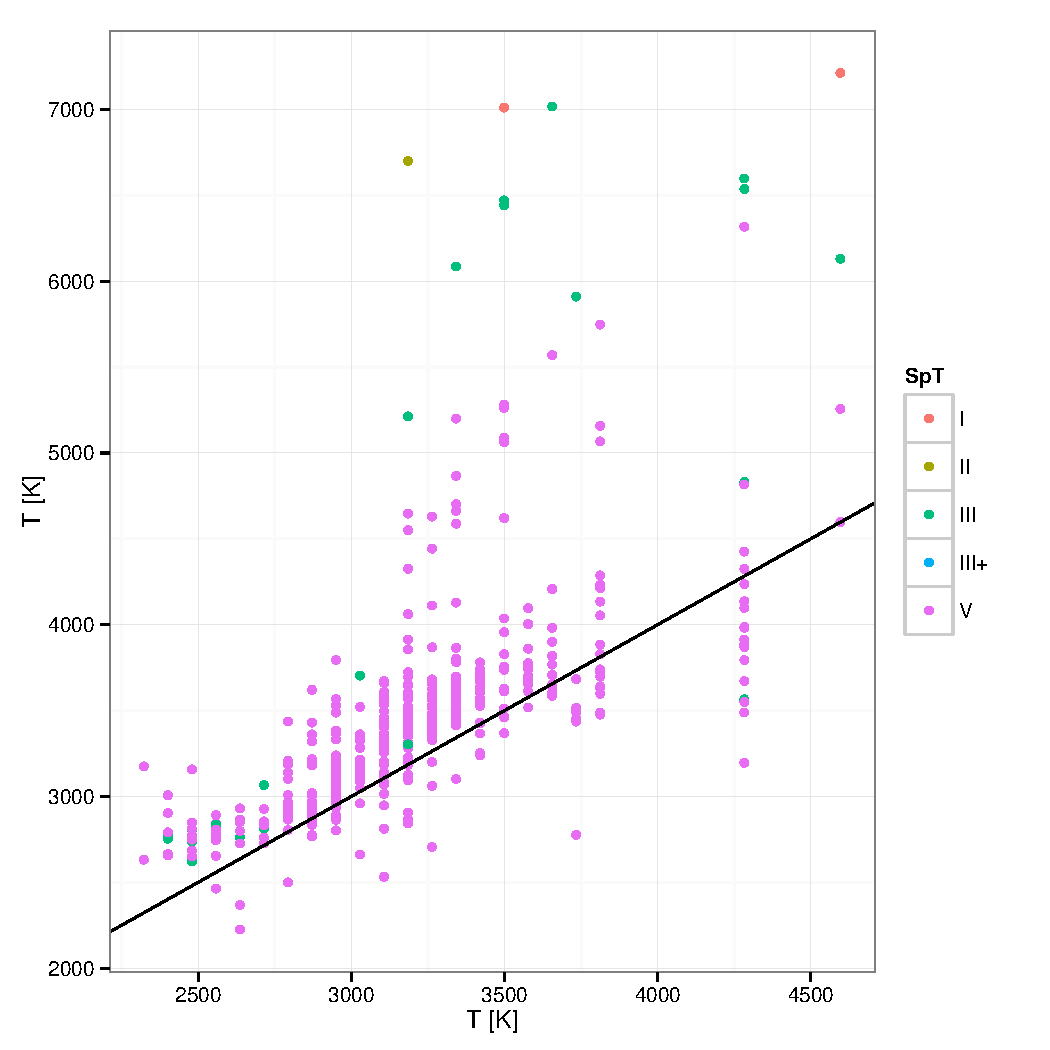
\includegraphics[width=6cm]{figs/T50GA_TSB.pdf}
 \caption{Comparison between Temperature estimations from Spectral Subtype 
 in x axis and the Random Forest for Ga based features trained with BT-Settl 
 at SNR=50 on y-axis}
 \label{fig:t50ga_tsb}
 \end{center}
\end {figure}

Similarly Figure~\ref{fig:t10ga_tsb} shows the relationship against GA features 
and Random Forest model trained by BT-Settl at SNR=10.
\begin {figure}
 \begin{center}
 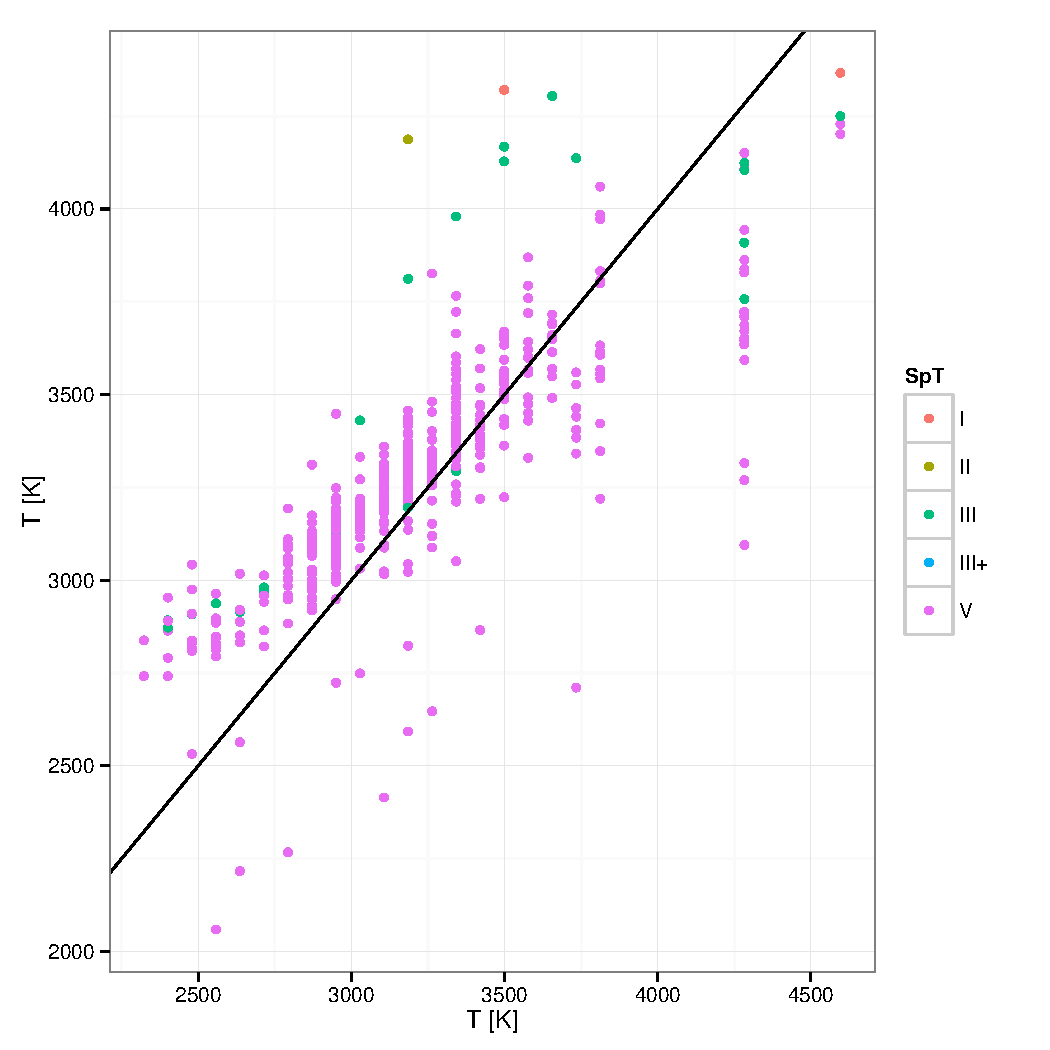
\includegraphics[width=6cm]{figs/T10GA_TSB.pdf}
 \caption{Comparison between Temperature estimations from Spectral Subtype 
 in x axis and the Random Forest for Ga based features trained with BT-Settl 
 at SNR=10 on y-axis}
 \label{fig:t10ga_tsb}
 \end{center}
\end {figure}

The same was made with features forposed by Cesetti et al. 
(see Figure~\ref{fig:t50cs_tsb} and Figure~\ref{fig:t10cs_tsb}).

\begin {figure}
 \begin{center}
 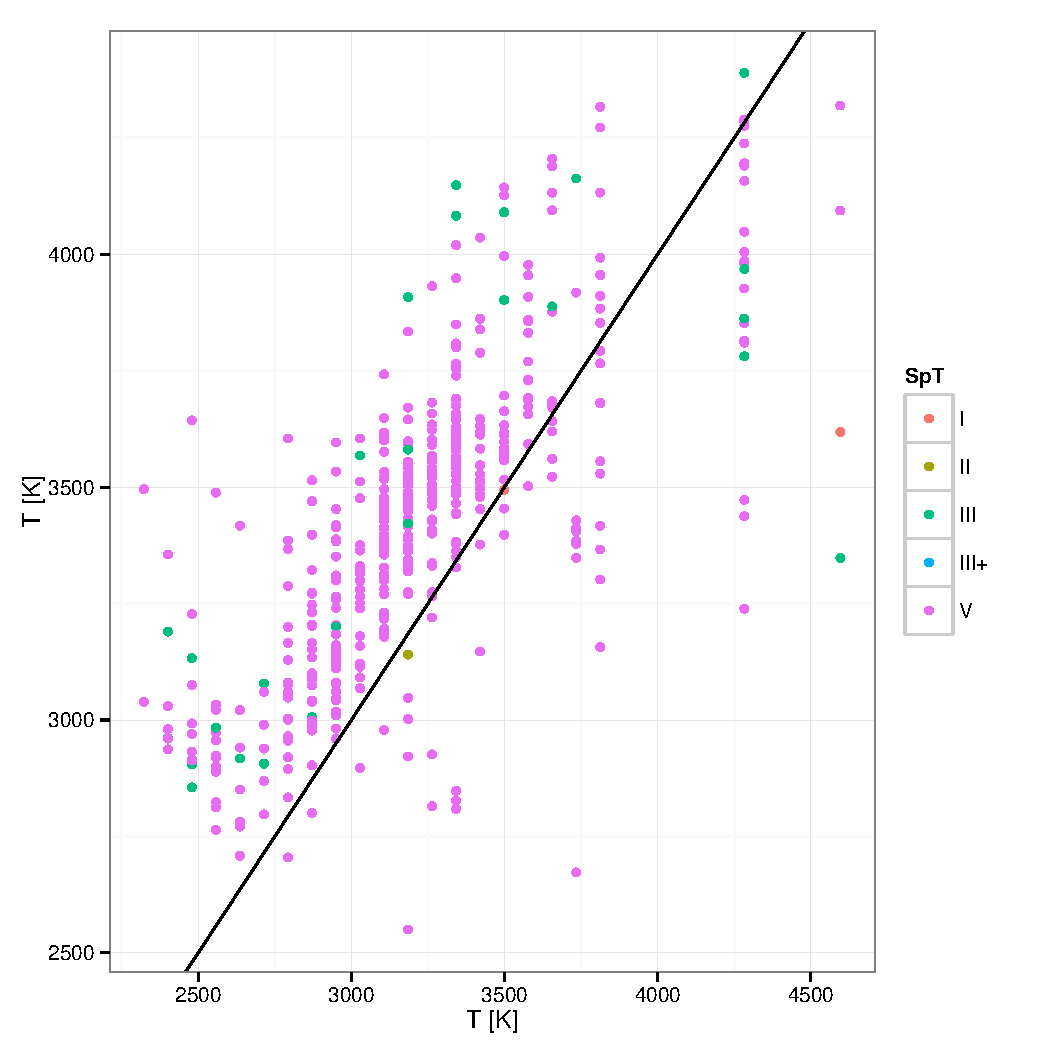
\includegraphics[width=6cm]{figs/T50CS_TSB.pdf}
 \caption{Comparison between Temperature estimations from Spectral Subtype 
 in x axis and the Random Forest for Cesetti et al. features trained with BT-Settl 
 at SNR=50 on y-axis}
 \label{fig:t50cs_tsb}
 \end{center}
\end {figure}

\begin {figure}
 \begin{center}
 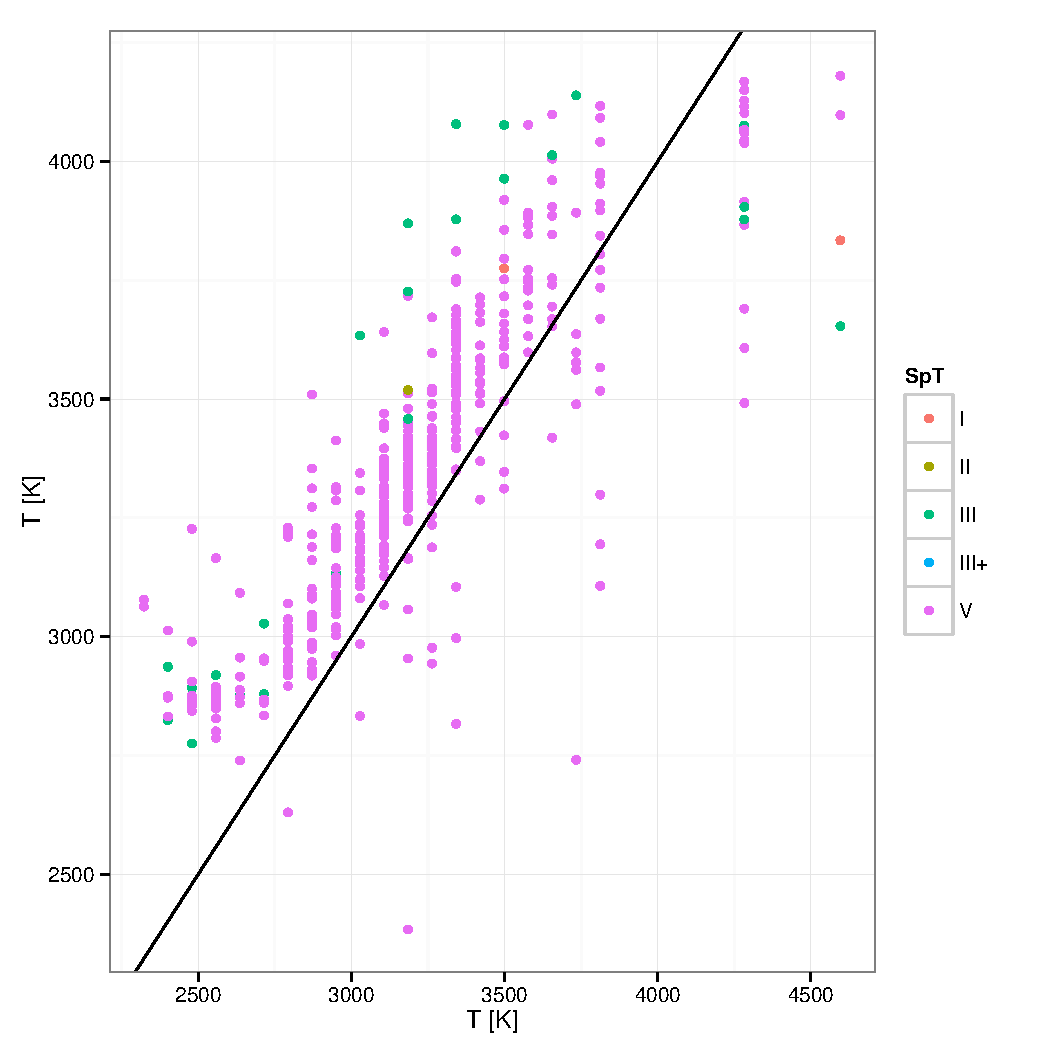
\includegraphics[width=6cm]{figs/T10CS_TSB.pdf}
 \caption{Comparison between Temperature estimations from Spectral Subtype 
 in x axis and the Random Forest for Cesetti et al. features trained with BT-Settl 
 at SNR=10 on y-axis}
 \label{fig:t10cs_tsb}
 \end{center}
\end {figure}

The analysis was done for Global spectrum based approach. 
Thus in Figure~\ref{fig:t50bp_tsb} and Figure~\ref{fig:t10bp_tsb} presents the relationship for 
the diemensional reduction and SVM approach and 
Figure~\ref{} and Figure~\ref{} accounts for similarity 
based estimation of pysical parameters accoding to $\chi^2$ metric.

\begin {figure}
 \begin{center}
 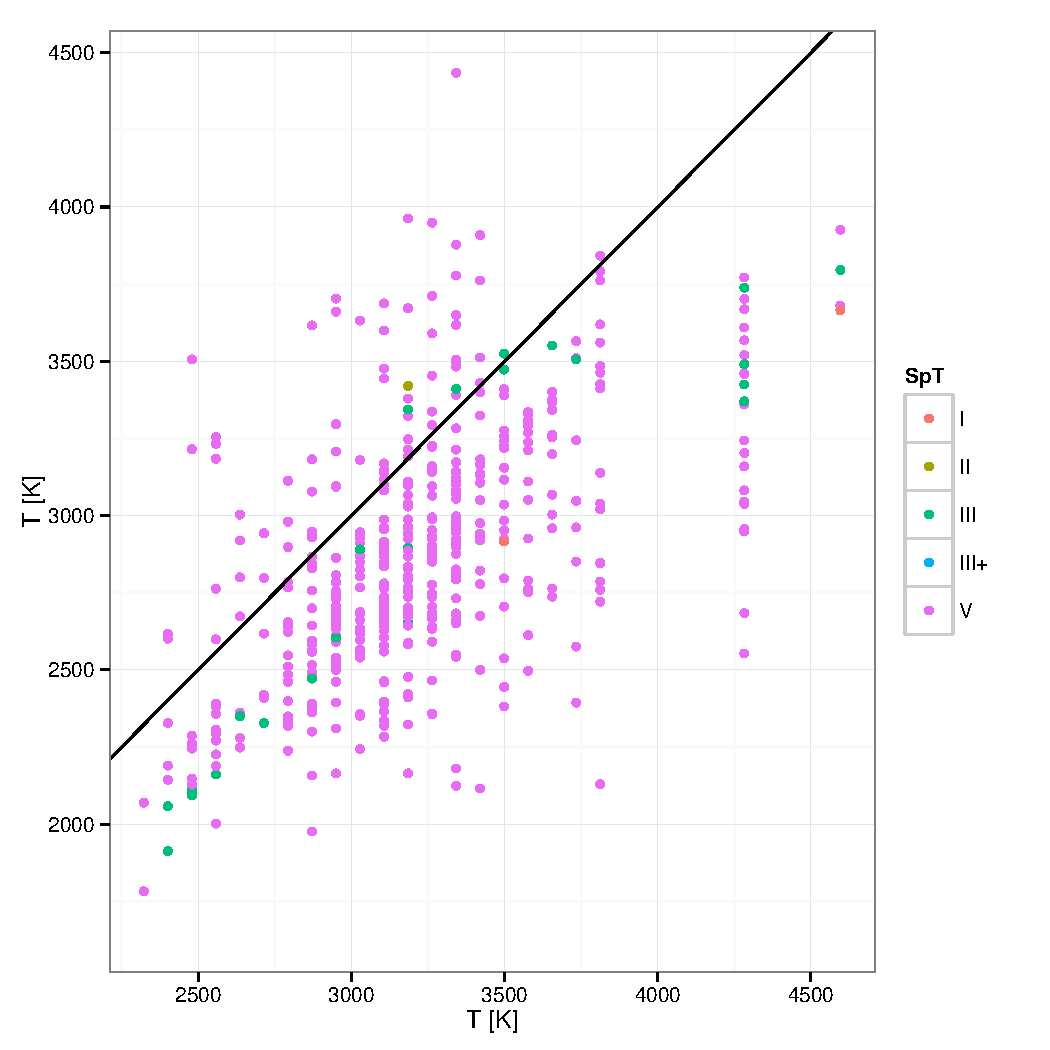
\includegraphics[width=6cm]{figs/T50BP_TSB.pdf}
 \caption{Comparison between Temperature estimations from Spectral Subtype 
 in x axis and the Random Forest for full length spectra trained with BT-Settl 
 at SNR=50 on y-axis}
 \label{fig:t50bp_tsb}
 \end{center}
\end {figure}

\begin {figure}
 \begin{center}
 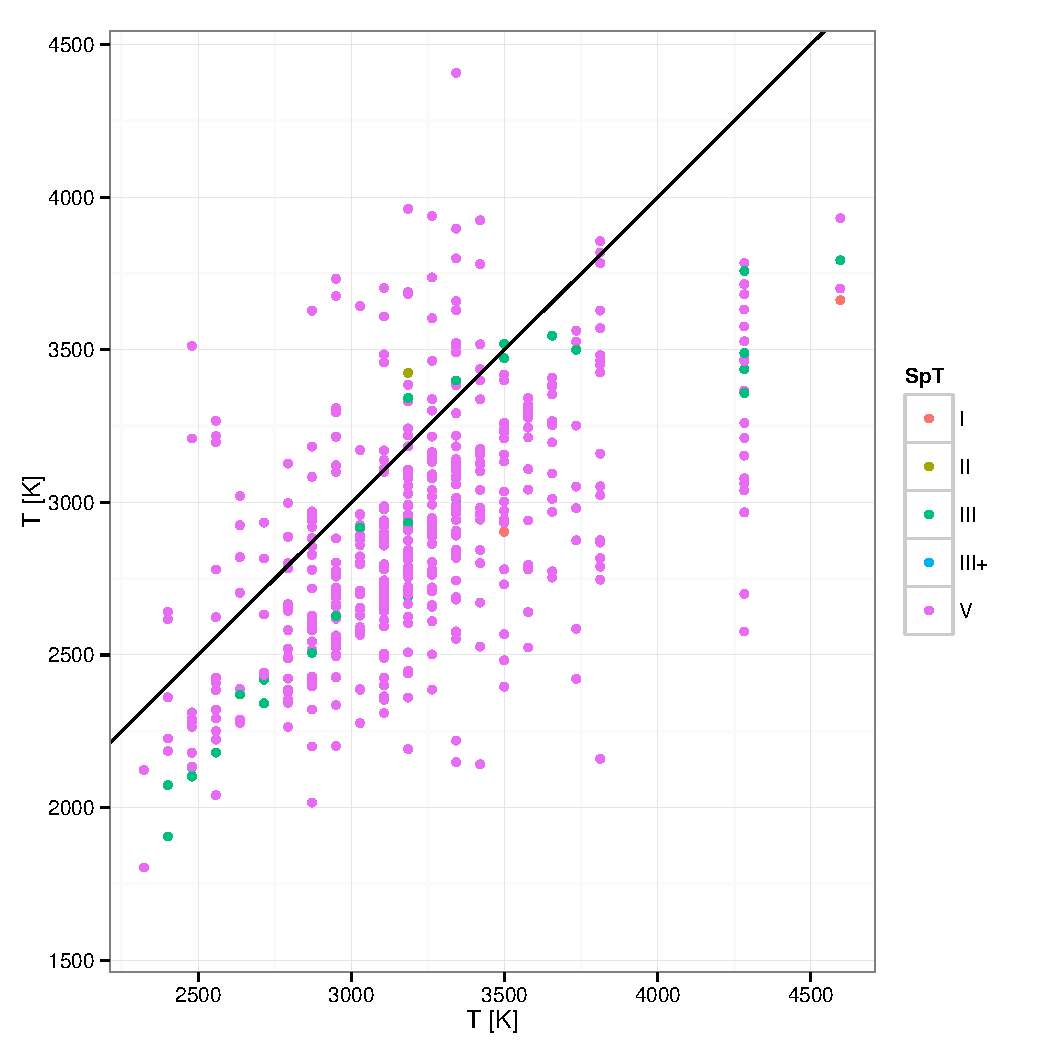
\includegraphics[width=6cm]{figs/T10BP_TSB.pdf}
 \caption{Comparison between Temperature estimations from Spectral Subtype 
 in x axis and the Random Forest for full length spectra trained with BT-Settl 
 at SNR=10 on y-axis}
 \label{fig:t10BP_tsb}
 \end{center}
\end {figure}

\begin {figure}
 \begin{center}
 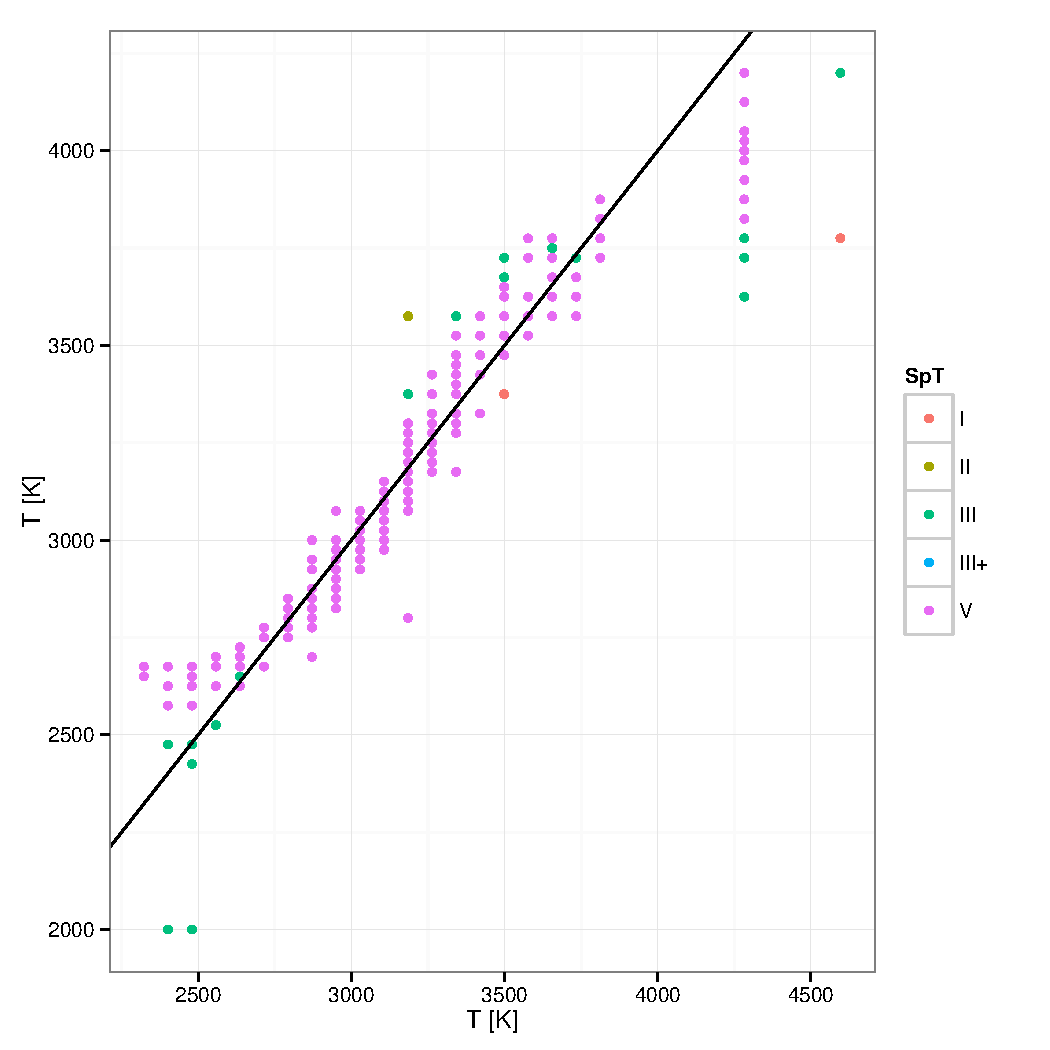
\includegraphics[width=6cm]{figs/T50CH_TSB.pdf}
 \caption{Comparison between Temperature estimations from Spectral Subtype 
 in x axis and the closest BT-Settl spectrum with SNR=50 on y-axis}
 \label{fig:t50bp_tsb}
 \end{center}
\end {figure}

\begin {figure}
 \begin{center}
 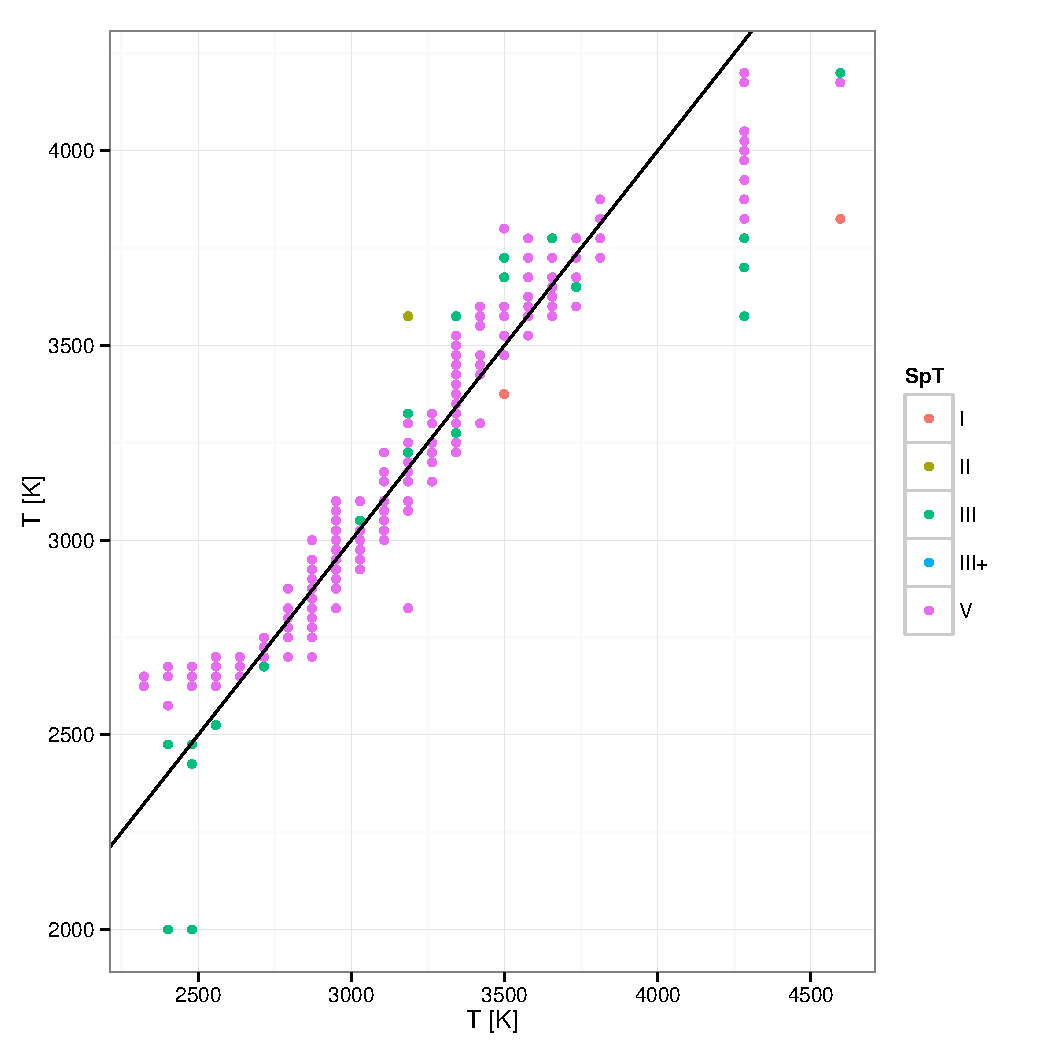
\includegraphics[width=6cm]{figs/T10CH_TSB.pdf}
 \caption{Comparison between Temperature estimations from Spectral Subtype 
 in x axis and the closest BT-Settl spectrum with SNR=10 on y-axis}
 \label{fig:t10BP_tsb}
 \end{center}
\end {figure}

% No le añado más discusión de momento, hasta ver si tiene sentido poer toda esta
% fila de gráficas o es mejor producir algo más condensado.
%
}


{
Te same approach can become useful to produce $log(gg)$ estimations. 
Here comparisons can only be possible between GA based features and
global spectra based approach.

In Figure~\ref{fig:Gbp_Gga_50} and Figure~\ref{fig:Gbp_Gga_10} 
relationships between $log(g)$ predicted by global espectrum estimation 
and GA feature based estimation can be observed.
Additionally Figure~\ref{fig:Gch_Gga_50} and Figure~\ref{fig:Gch_Gga_10}
present the relationship between the GA based estimation and the 
$\chi^2$ nearest BT-Settl spectrum.

\begin {figure}
 \begin{center}
 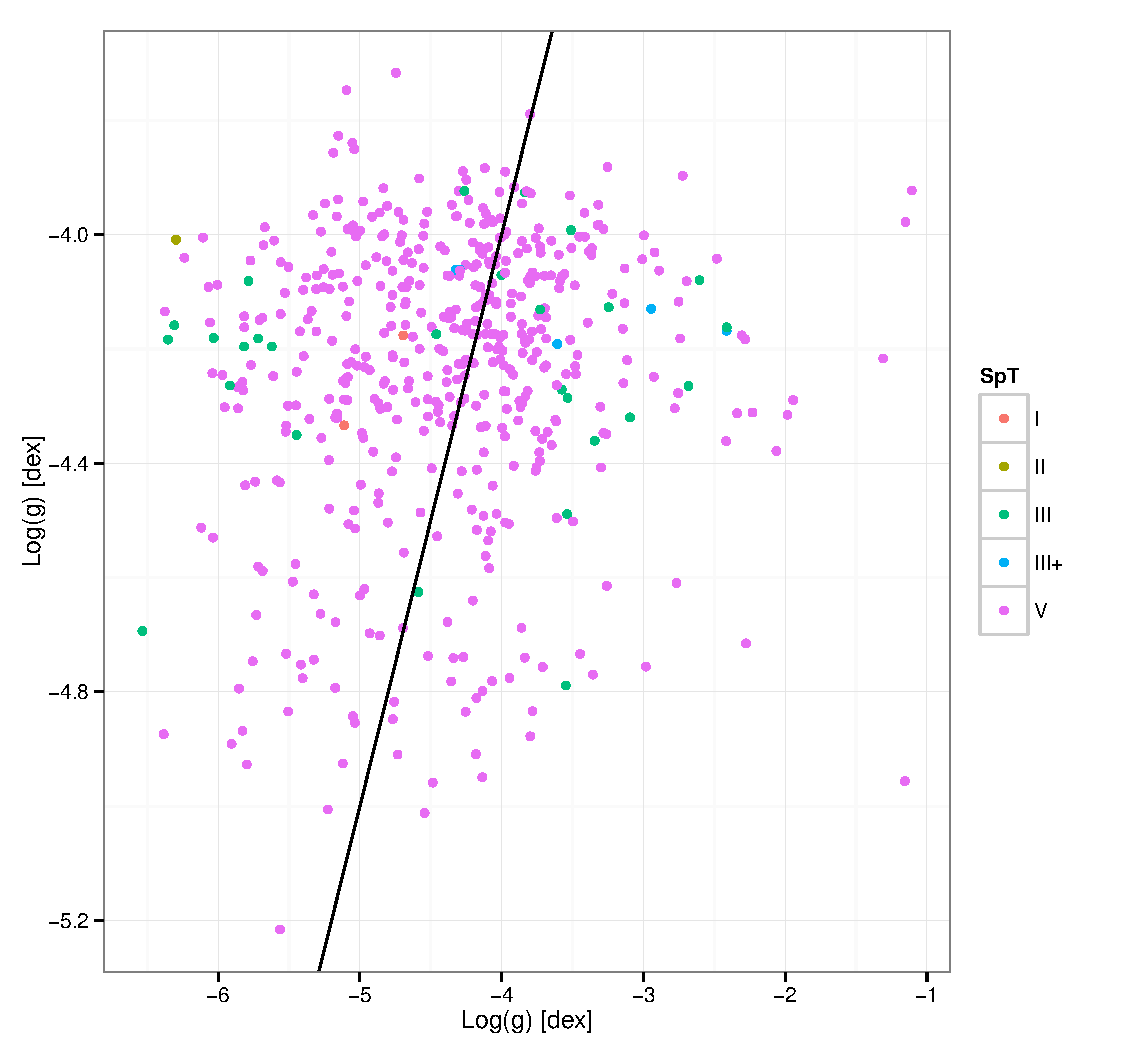
\includegraphics[width=6cm]{figs/LGBP_LGGA_50.pdf}
 \caption{Comparison between $log(g)$ estimations from 
 Random Forest model using GA features  in x axis and 
 the Global projected spectrum (ICA+SVM) with SNR=50 on y-axis}
 \label{fig:Gbp_Gga_50}
 \end{center}
\end {figure}

\begin {figure}
 \begin{center}
 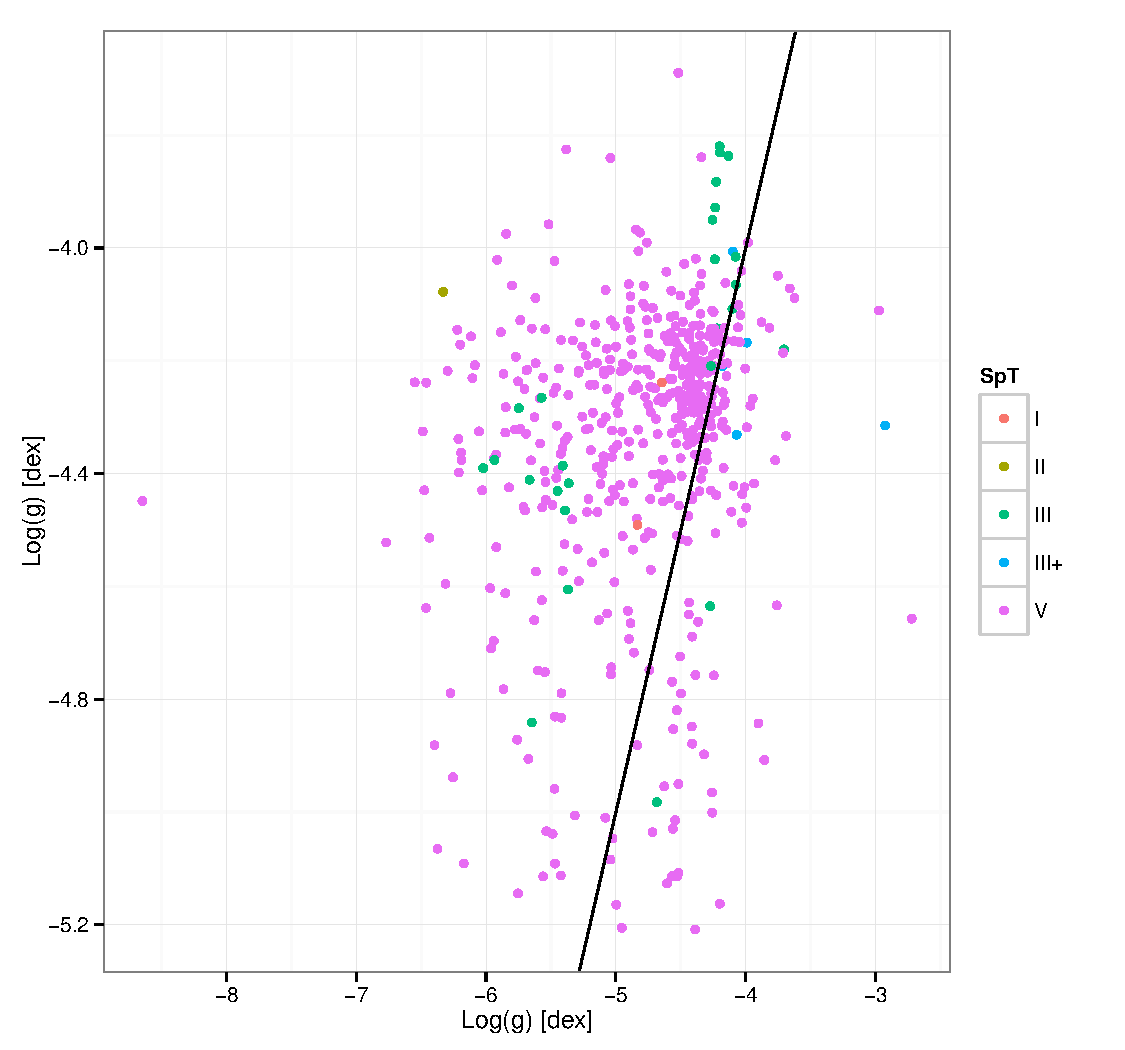
\includegraphics[width=6cm]{figs/LGBP_LGGA_10.pdf}
 \caption{Comparison between $log(g)$ estimations from 
 Random Forest model using GA features  in x axis and 
 the Global projected spectrum (ICA+SVM) with SNR=10 on y-axis}
 \label{fig:Gbp_Gga_10}
 \end{center}
\end {figure}

\begin {figure}
 \begin{center}
 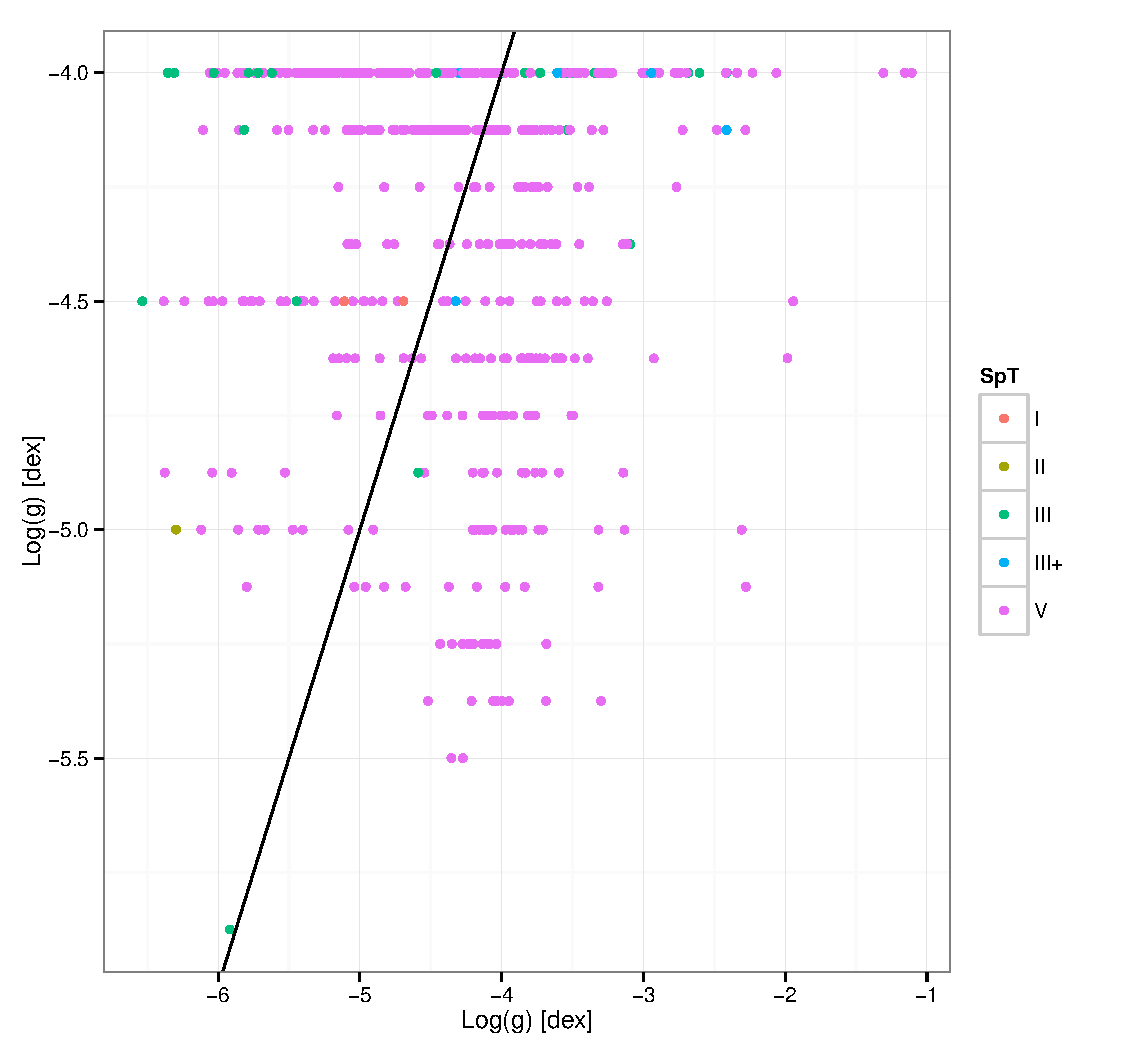
\includegraphics[width=6cm]{figs/LGCH_LGGA_50.pdf}
 \caption{Comparison between $log(g)$ estimations from 
 Random Forest model using GA features  in x axis and 
 the nearest $\chi^2$ BT-Settl spectrum with SNR=10 on y-axis}
 \label{fig:Gch_Gga_50}
 \end{center}
\end {figure}

\begin {figure}
 \begin{center}
 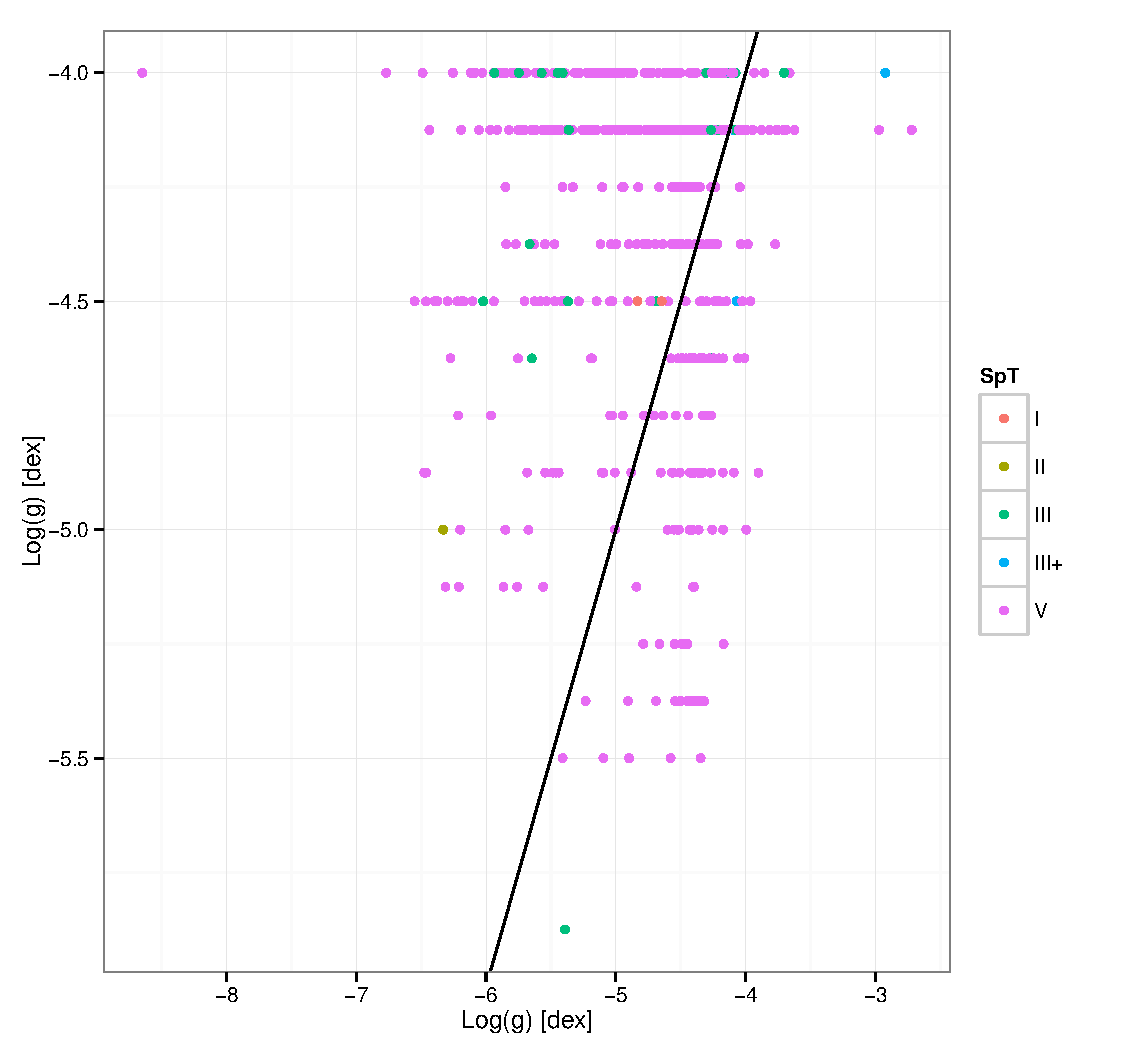
\includegraphics[width=6cm]{figs/LGCH_LGGA_10.pdf}
 \caption{Comparison between $log(g)$ estimations from 
 Random Forest model using GA features  in x axis and 
 the nearest $\chi^2$ BT-Settl spectrum with SNR=10 on y-axis}
 \label{fig:Gch_Gga_10}
 \end{center}
\end {figure}

% De nuevo las valoraciones deberían esperar a ver qué ponemos.

}

{ 

Finally, the same analysis is performed for the Metallicty parameter

\begin {figure}
 \begin{center}
 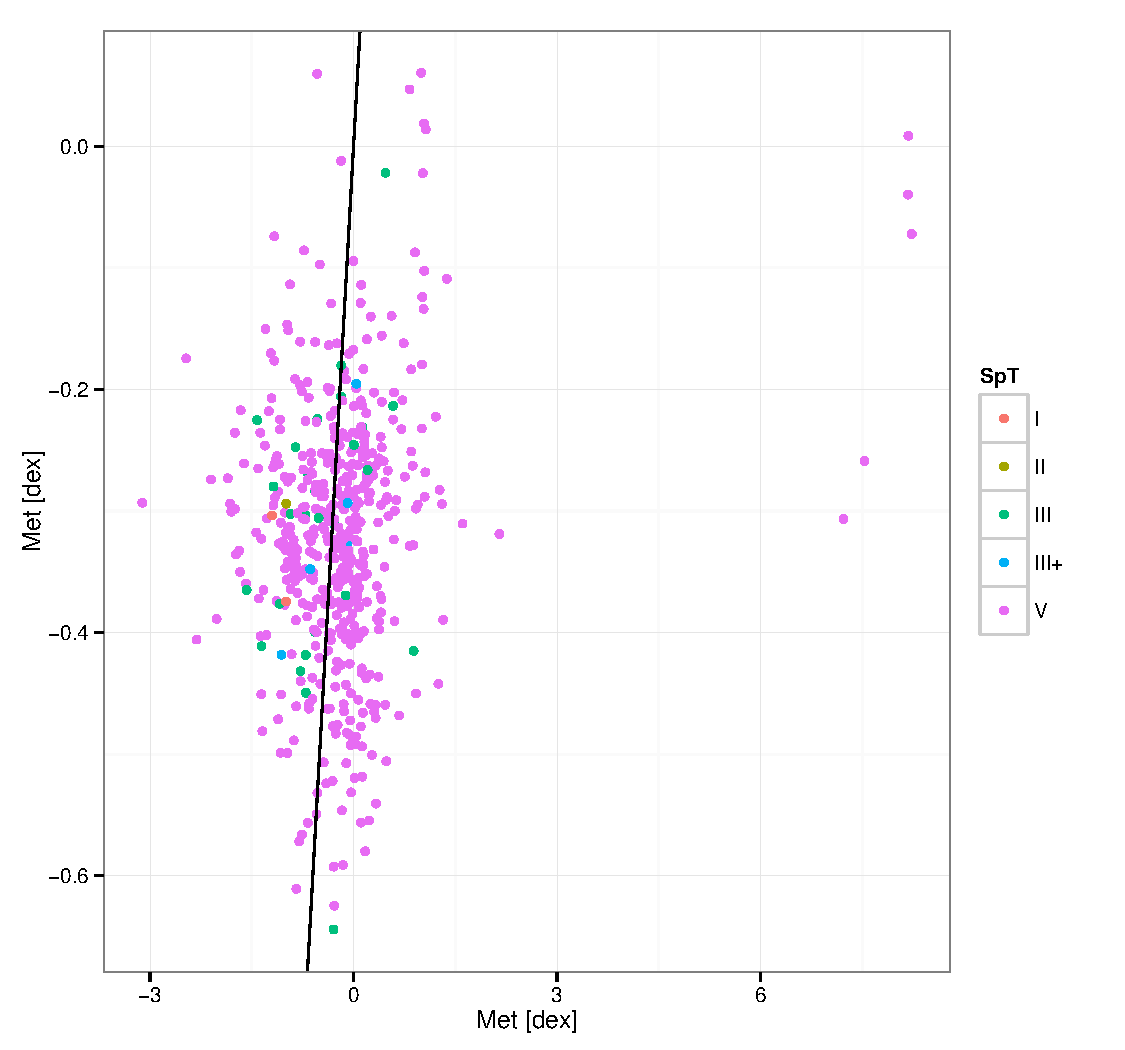
\includegraphics[width=6cm]{figs/MBP_MGA_50.pdf}
 \caption{Comparison between Metallicity estimations from 
 Random Forest model using GA features  in x axis and 
 the Global projected spectrum (ICA+SVM) with SNR=50 on y-axis}
 \label{fig:Mbp_Mga_50}
 \end{center}
\end {figure}

\begin {figure}
 \begin{center}
 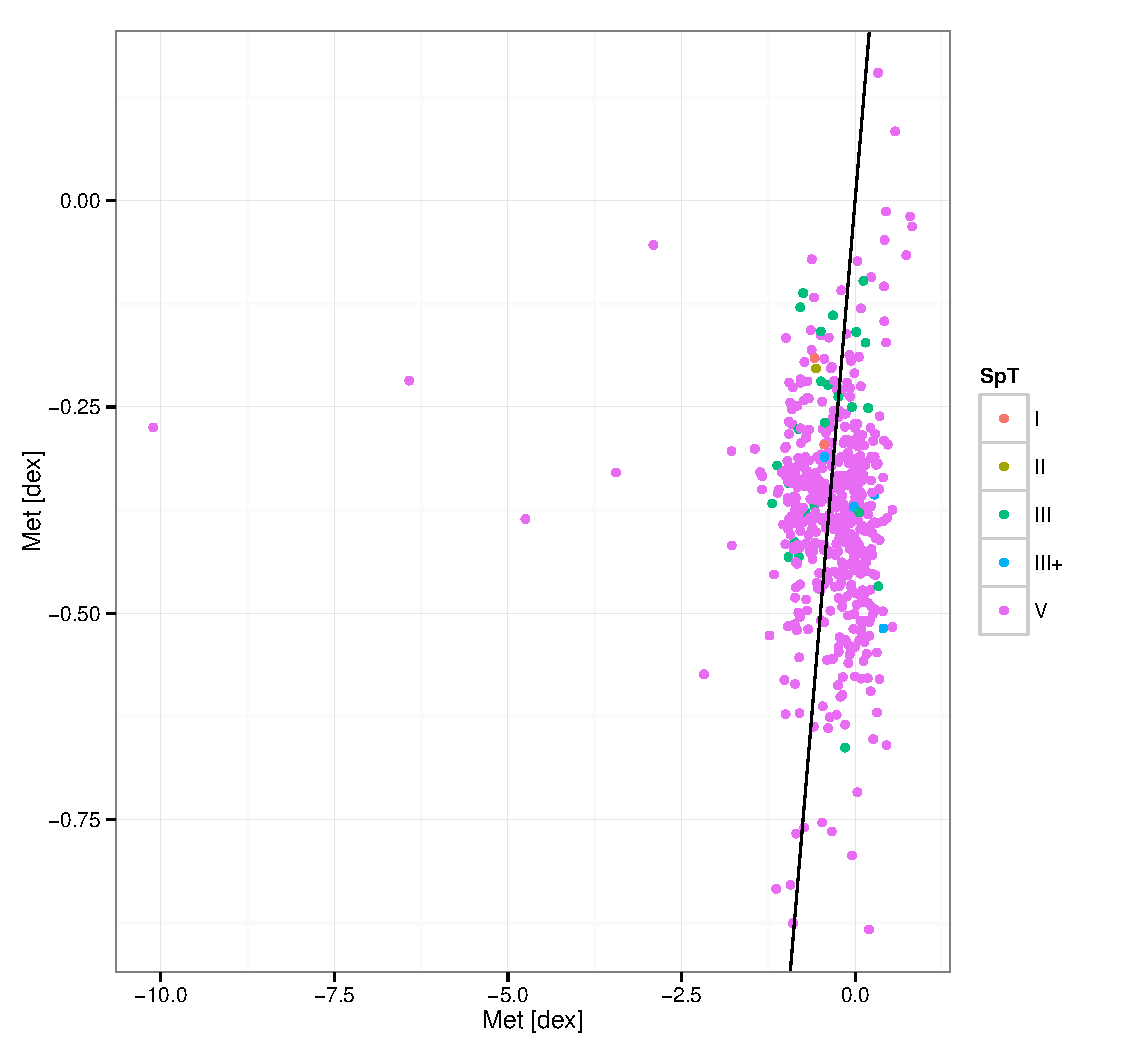
\includegraphics[width=6cm]{figs/MBP_MGA_10.pdf}
 \caption{Comparison between Metallicity estimations from 
 Random Forest model using GA features  in x axis and 
 the Global projected spectrum (ICA+SVM) with SNR=10 on y-axis}
 \label{fig:Mbp_Mga_10}
 \end{center}
\end {figure}

\begin {figure}
 \begin{center}
 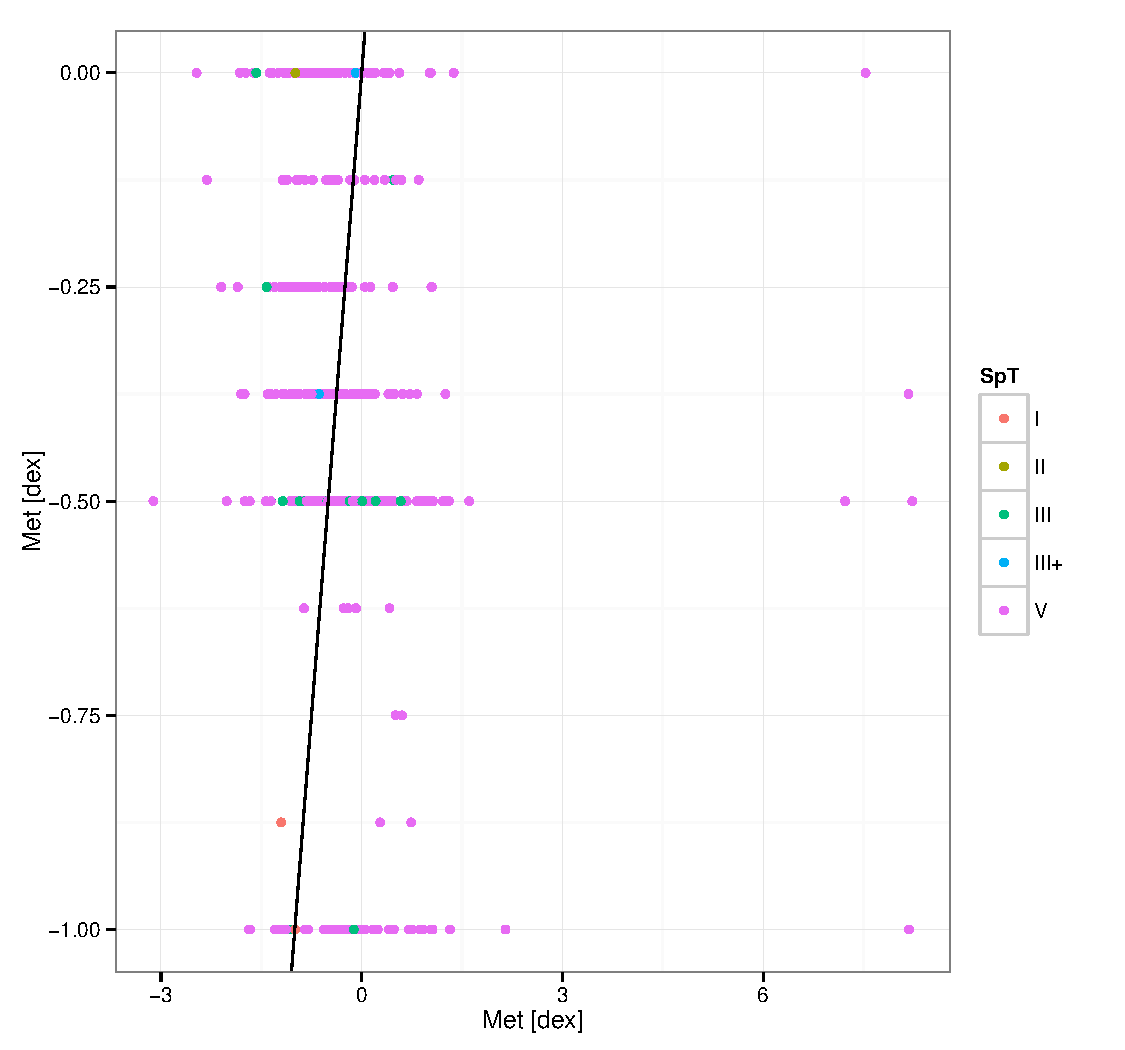
\includegraphics[width=6cm]{figs/MCH_MGA_50.pdf}
 \caption{Comparison between Metallicity estimations from 
 Random Forest model using GA features  in x axis and 
 the nearest $\chi^2$ BT-Settl spectrum with SNR=10 on y-axis}
 \label{fig:Mch_Mga_50}
 \end{center}
\end {figure}

\begin {figure}
 \begin{center}
 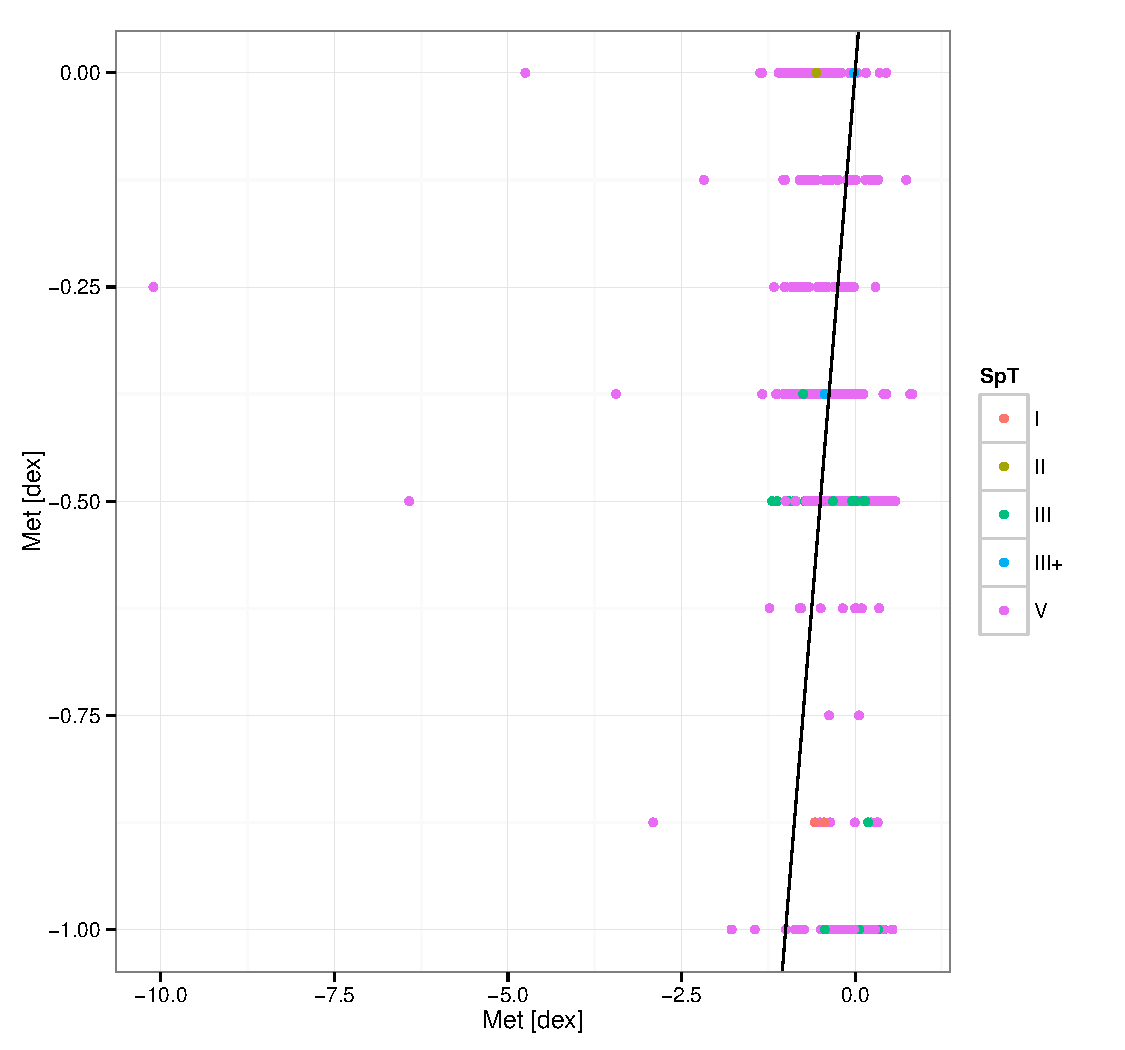
\includegraphics[width=6cm]{figs/MCH_MGA_10.pdf}
 \caption{Comparison between Metallicity estimations from 
 Random Forest model using GA features  in x axis and 
 the nearest $\chi^2$ BT-Settl spectrum with SNR=10 on y-axis}
 \label{fig:Mch_Mga_10}
 \end{center}
\end {figure}

% De nuevo, el análisis y discusión, función de lo que queramos dejar
}

{
It is possible to present relationships between $log(g)$ and $log(T_{eff})$
as a matter of congruence analysis between predictions.

\begin{figure}
 \begin{center}
 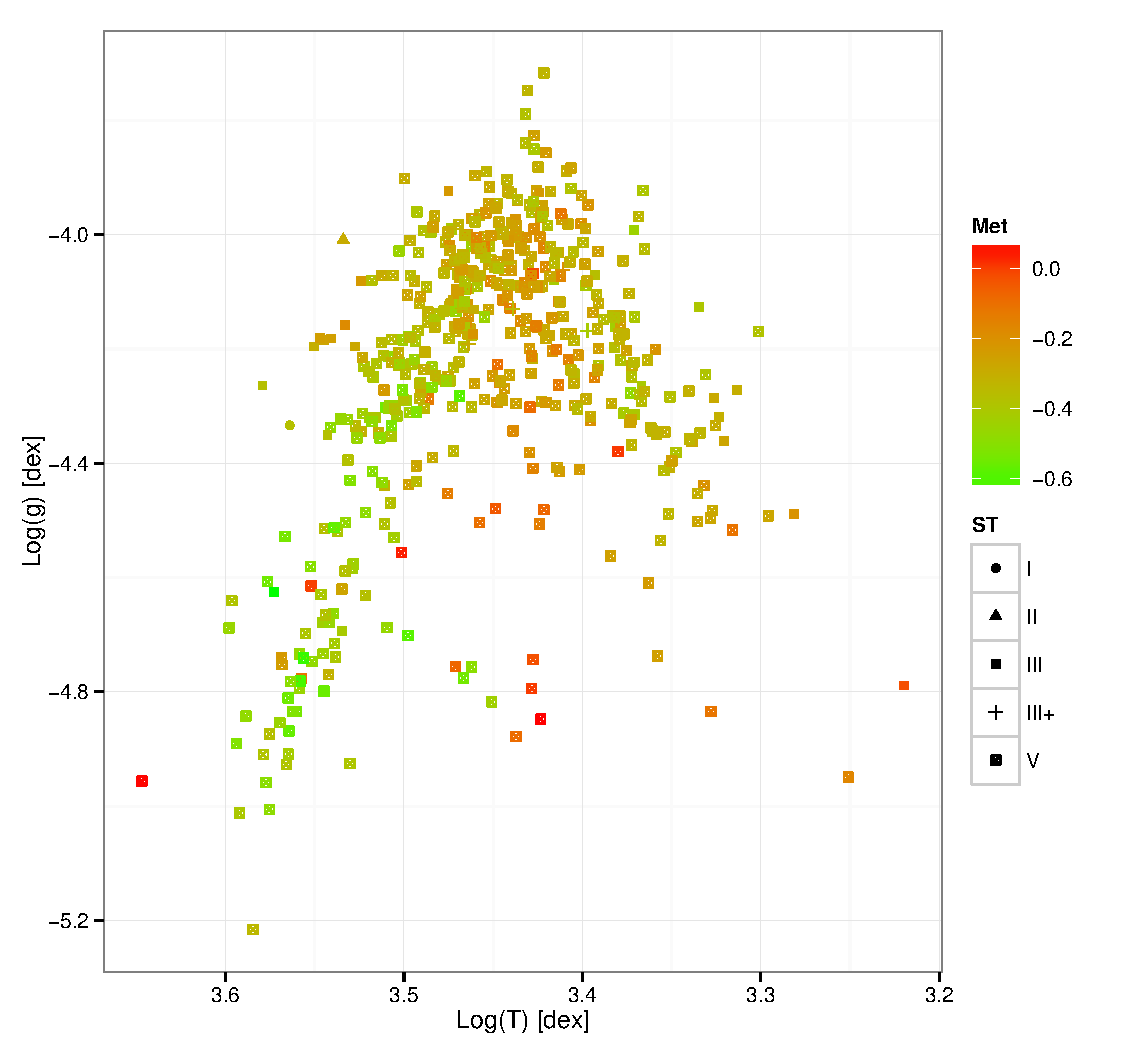
\includegraphics[width=6cm]{figs/LG_LT_BP_50.pdf}
 \caption{Relationship between $log(T_{eff}) $ in the x axis 
 and $log(g)$ in the y axis for SNR=50 when Global ICA+SVM model
 is used}
 \label{fig:lg_lt_bp_50}
 \end{center}
\end{figure}

\begin{figure} 
 \begin{center}
 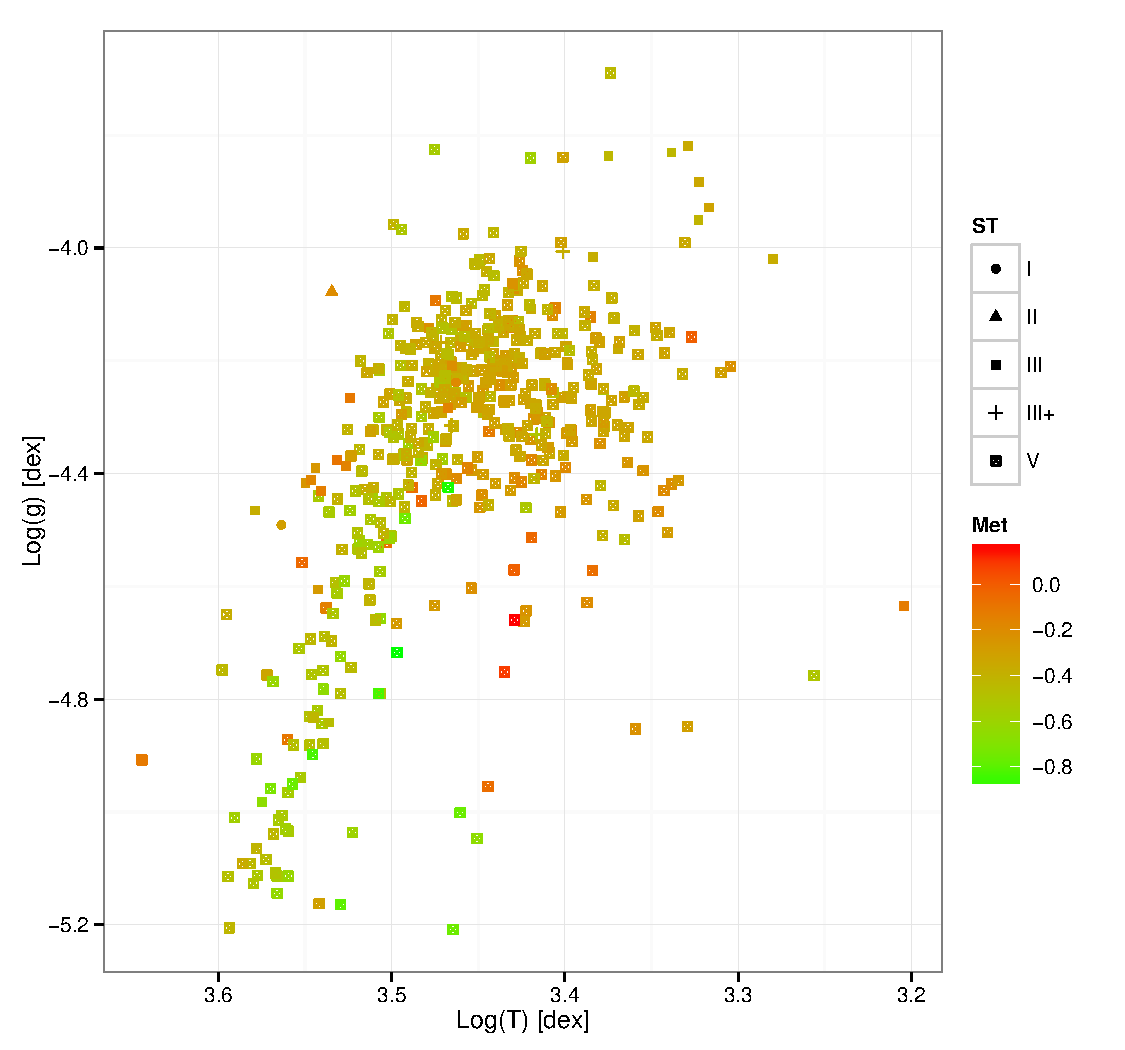
\includegraphics[width=6cm]{figs/LG_LT_BP_10.pdf}
 \caption{Relationship between $log(T_{eff}) $ in the x axis 
 and $log(g)$ in the y axis for SNR=10 when Global ICA+SVM model
 is used}
 \label{fig:lg_lt_bp_50}
 \end{center}
\end{figure}

The same can be performed when the estimations arise from models 
based on features provided by the GA technique.

\begin{figure}
 \begin{center}
 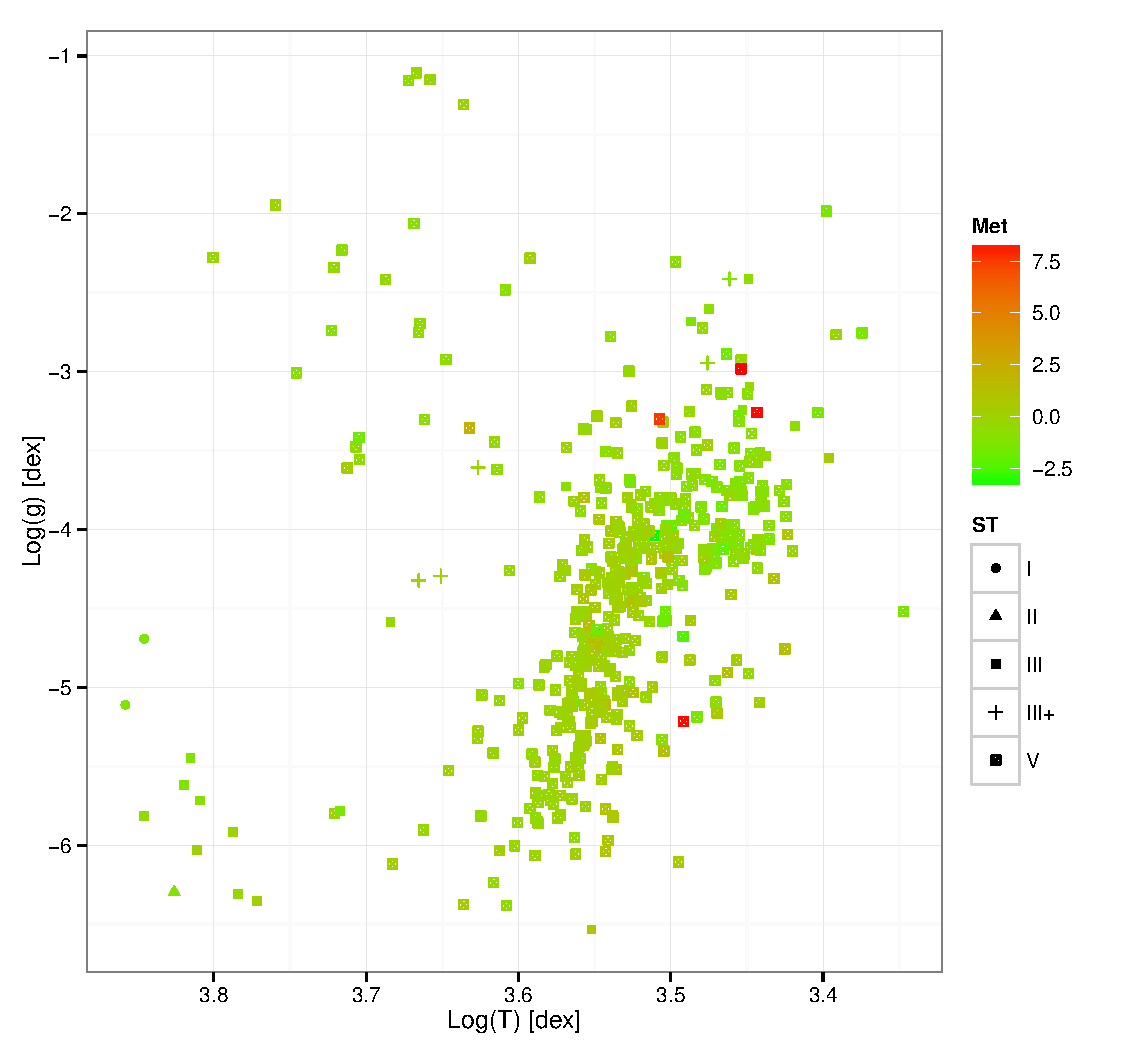
\includegraphics[width=6cm]{figs/LG_LT_GA_50.pdf}
 \caption{Relationship between $log(T_{eff}) $ in the x axis 
 and $log(g)$ in the y axis for SNR=50 when 
 the Random Forest model over the GA provided features 
 is used}
 \label{fig:lg_lt_ga_50}
 \end{center}
\end{figure}

\begin{figure}
 \begin{center}
 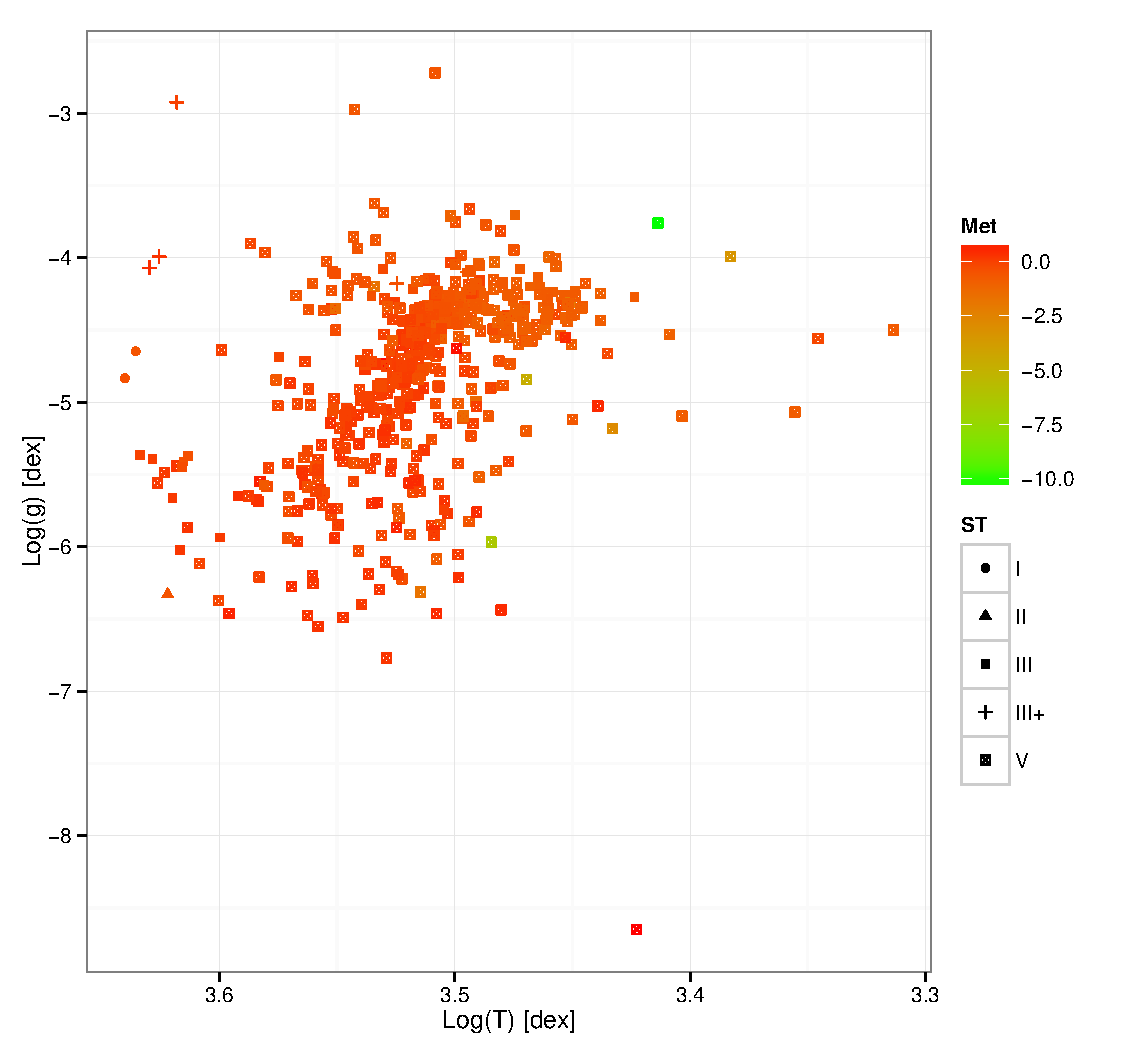
\includegraphics[width=6cm]{figs/LG_LT_GA_10.pdf}
 \caption{Relationship between $log(T_{eff}) $ in the x axis 
 and $log(g)$ in the y axis for SNR=10 when 
 the Random Forest model over the GA provided features 
 is used}
 \label{fig:lg_lt_ga_10}
 \end{center}
\end{figure}


And, for sure, it is possible to do it for estimations based on 
parameters from nearest labeled BT-Settl spectra.
In this particular case, it is possible to see how 
considering the global spectrum is positive for stronger 
physical parameters like $T_{eff}$ but the approach
reduces drastically its likelihood when other softer 
parameters are involved.

\clearpage 

\begin{figure}
 \begin{center}
 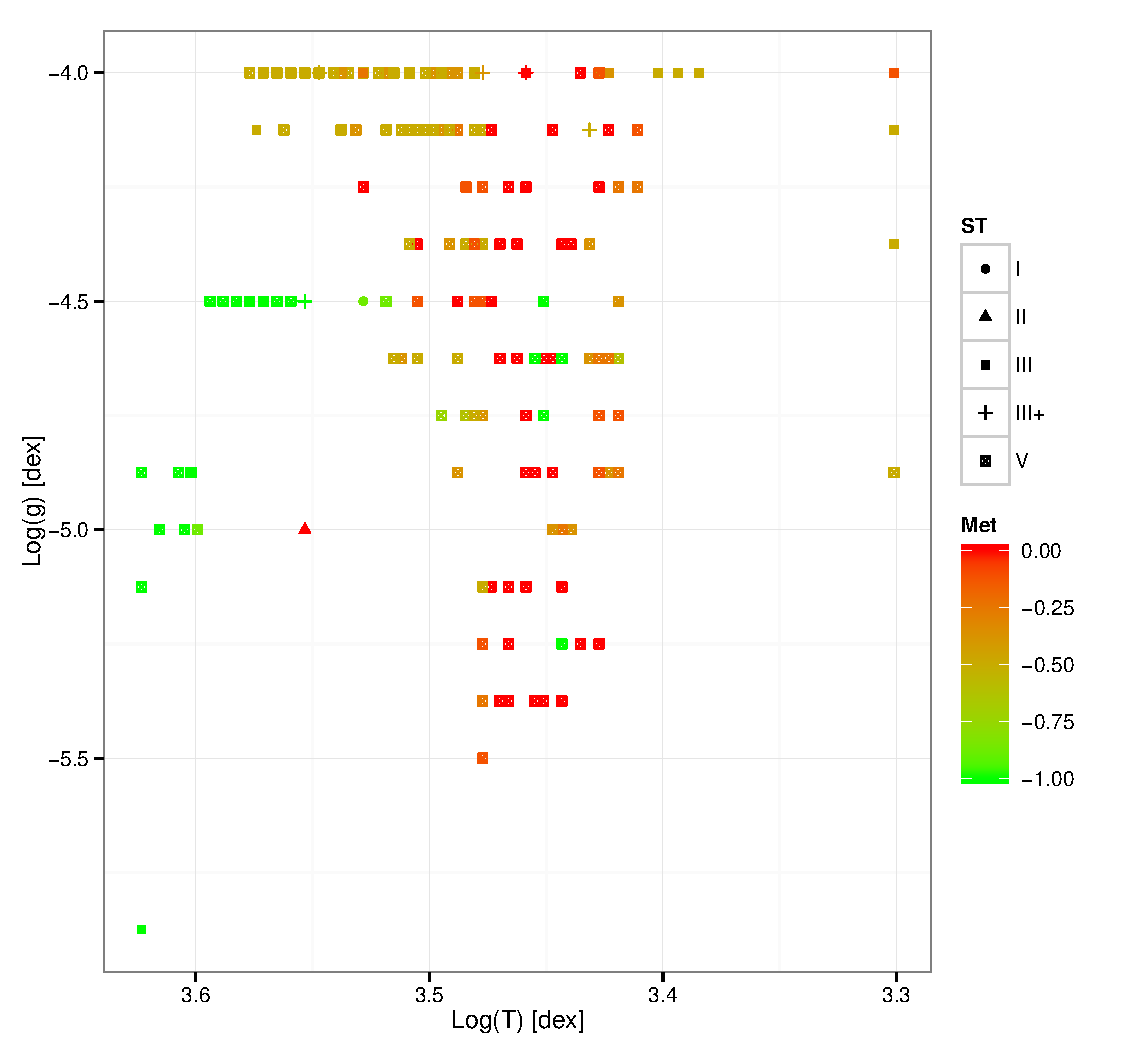
\includegraphics[width=6cm]{figs/LG_LT_CH_50.pdf}
 \caption{Relationship between $log(T_{eff}) $ in the x axis 
 and $log(g)$ in the y axis for SNR=50 when 
 the nearest BT-Settl spectrum is used}
 \label{fig:lg_lt_ch_50}
 \end{center}
\end{figure}

In the end deeper analysis needs to be carried out considering
several factors like coherence between labeled referenced 
library spectrum, density of the labeled spectra, etc.

\begin{figure}
 \begin{center}
 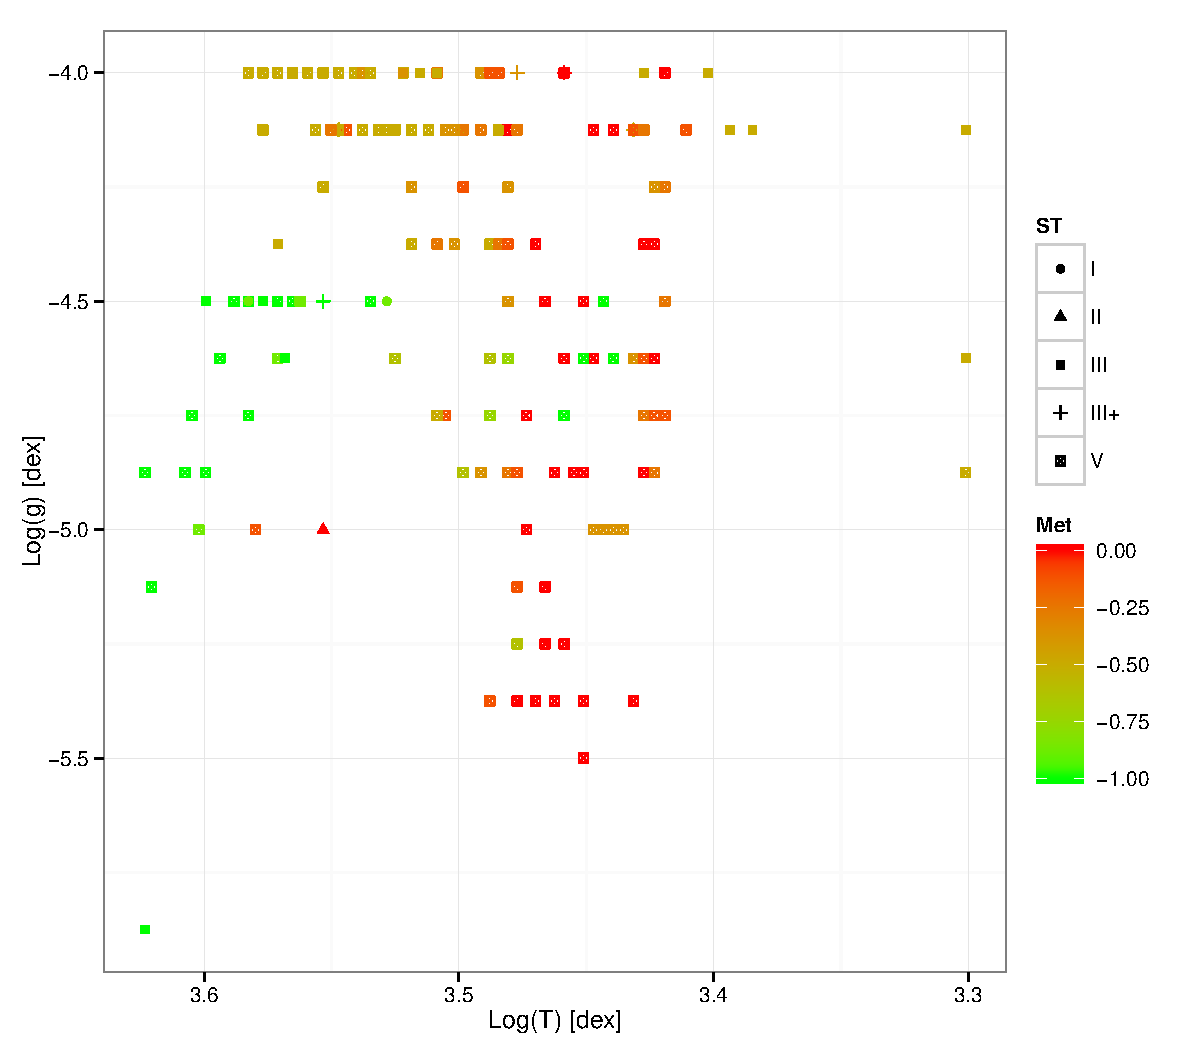
\includegraphics[width=6cm]{figs/LG_LT_CH_10.pdf}
 \caption{Relationship between $log(T_{eff}) $ in the x axis 
 and $log(g)$ in the y axis for SNR=10 when 
 the nearest BT-Settl spectrum is used}
 \label{fig:lg_lt_ch_10}
 \end{center}
\end{figure}


}

\section{Distribution of predicted parameters.}
\input{predictions}

\section{Conclusions}

\begin{acknowledgements}
This research has benefitted from the M, L, T, and Y dwarf compendium housed at DwarfArchives.org.
The authors also thanks to the Spanish Ministery for Economy and Innovation because of the 
support obtained through the project with ID: AyA2011-24052. IRTF library provided by the 
University of Hawaii under Cooperative Agreement no. NNX-08AE38A with the National 
Aeronautics and Space Administration, Science Mission Directorate, Planetary Astronomy Program.
\end{acknowledgements}

%-------------------------------------------------------------------

\bibliography{references_m}{}
\bibliographystyle{bibtex/aa}

\end{document}
